%==========================================================================
% PrivFed-TCN: Privacy-Preserving Federated Learning IDS for IoT Networks
% IEEE Conference Paper - ready for Overleaf
%
% Compile with pdflatex (twice) + bibtex (or run latexmk -pdf).
%
% Required Overleaf packages: IEEEtran, graphicx, amsmath, amssymb,
% booktabs, multirow, array, hyperref, url, tikz, pgfplots, listings, xcolor.
% These are all bundled with TeX Live / Overleaf default.
%==========================================================================
\documentclass[conference]{IEEEtran}
\IEEEoverridecommandlockouts

% ---------- Packages -----------------------------------------------------
\usepackage{cite}
\usepackage{amsmath,amssymb,amsfonts}
\usepackage{algorithmic}
\usepackage{graphicx}
\usepackage{textcomp}
\usepackage{xcolor}
\usepackage{booktabs}
\usepackage{multirow}
\usepackage{array}
\usepackage{url}
\usepackage{hyperref}
\usepackage{tikz}
\usetikzlibrary{shapes.geometric, arrows.meta, positioning, fit, backgrounds, calc}
\usepackage{pgfplots}
\pgfplotsset{compat=1.17}

% Better-looking inline math symbols
\newcommand{\eps}{\varepsilon}

% Hyperref styling
\hypersetup{
  colorlinks=true,
  linkcolor=black,
  citecolor=blue,
  urlcolor=blue
}

\def\BibTeX{{\rm B\kern-.05em{\sc i\kern-.025em b}\kern-.08em
    T\kern-.1667em\lower.7ex\hbox{E}\kern-.125emX}}

\begin{document}

% ---------- Title --------------------------------------------------------
\title{PrivFed-TCN: A Privacy-Preserving Federated Learning Intrusion
       Detection System for IoT Networks Using Temporal Convolutional
       Networks}

\author{
  \IEEEauthorblockN{Ahmed Mujtaba}
  \IEEEauthorblockA{Department of Artificial Intelligence\\
                    FAST NUCES, Islamabad, Pakistan\\
                    i220470@nu.edu.pk}
  \and
  \IEEEauthorblockN{Safwan Hafeez}
  \IEEEauthorblockA{Department of Artificial Intelligence\\
                    FAST NUCES, Islamabad, Pakistan\\
                    i220588@nu.edu.pk}
}

\maketitle

% ---------- Abstract -----------------------------------------------------
\begin{abstract}
The proliferation of Internet of Things (IoT) devices has created vast
attack surfaces susceptible to distributed denial-of-service (DDoS)
attacks, botnets, and malware. Traditional centralised Intrusion
Detection Systems (IDS) fail to scale with distributed IoT
architectures and expose sensitive telemetry during training. Federated
Learning (FL) addresses the privacy challenge by keeping raw traffic
on-device, but most existing FL-IDS pipelines rely on Long
Short-Term Memory (LSTM) networks that impose prohibitive compute
demands on resource-constrained nodes and lack formal privacy
guarantees against gradient-inversion attacks.
This paper proposes \textbf{PrivFed-TCN}, a privacy-preserving FL-IDS
that replaces LSTM with a compact Temporal Convolutional Network
augmented by multi-head self-attention, combined with R\'enyi
Differential Privacy (RDP) noise injection inside a hierarchical
FedProx aggregation pipeline. We evaluate the framework on the
CIC-IoT-2023 dataset across 14 attack classes under a strict shared
privacy budget of $\eps\!\le\!1.0$ ($\delta\!=\!10^{-5}$).
PrivFed-TCN attains \textbf{79.66\,\% test accuracy}, \textbf{0.586
F1-macro}, and \textbf{1.62\,\% false-positive rate}, beating an
identically DP-protected FL-LSTM baseline by \textbf{$+3.36$\,pp
accuracy} and \textbf{$+0.038$ F1} while transmitting \textbf{65.8\,\%
less data per round} (2.99 vs.\ 8.73 MB). To our knowledge this is the
first general-purpose FL-IDS that simultaneously demonstrates an
empirically calibrated $\eps\!\le\!1.0$ budget, a TCN-based model
fewer than 80\,K parameters, and a strict-privacy-fair comparison
against an LSTM baseline on a 14-class IoT attack taxonomy.
\end{abstract}

\begin{IEEEkeywords}
Federated Learning, Intrusion Detection System, Internet of Things,
Temporal Convolutional Network, Differential Privacy, Non-IID Data,
CIC-IoT-2023.
\end{IEEEkeywords}

% =========================================================================
\section{Introduction}\label{sec:intro}
The Internet of Things (IoT) has become one of the most transformative
technological paradigms of the twenty-first century. Smart homes,
industrial sensors, wearables, and vehicular networks now constitute
billions of connected endpoints that continuously generate, transmit,
and consume data. Forecasts project the global IoT device count will
exceed 30 billion by 2030, turning IoT ecosystems into critical
infrastructure underpinning healthcare, energy, logistics, and national
security. This explosive growth has expanded the cybersecurity threat
landscape commensurately. IoT devices are inherently heterogeneous in
processing capability, energy budget, and protocol stack, making
uniform security postures difficult to enforce.

Intrusion Detection Systems (IDS) are a foundational defence
mechanism. By monitoring traffic patterns and flagging deviations from
normal behaviour, an IDS can detect a wide spectrum of attacks ranging
from volumetric DDoS floods to stealthy botnet command-and-control
communication. Classical IDS architectures, however, presuppose a
centralised topology in which raw packets from every endpoint are
forwarded to a central server. This is untenable in IoT settings
because (i)~the volume of traffic generated by billions of endpoints
overwhelms centralised processing capacity, (ii)~routing raw sensor
data to a remote server constitutes a serious privacy violation and
conflicts with regulations such as GDPR, and (iii)~single-server
topologies introduce a single point of failure.

Federated Learning (FL), introduced by McMahan et al.~\cite{mcmahan2017},
decouples model training from data centralisation. Each device trains
a local model on its own data and transmits only parameter updates,
which a central aggregator averages into a global model. Because raw
data never leaves the device, FL inherently satisfies data
minimisation. The seminal work of Anwar et al.~\cite{anwar2025}
demonstrated FL coupled with LSTM networks for IoT intrusion
detection. However, three gaps persist:
\begin{itemize}
\item LSTM's recurrent structure imposes substantial compute and
      memory cost that constrained IoT nodes cannot sustain.
\item No formal differential-privacy guarantee is provided, leaving
      gradient updates susceptible to gradient-inversion attacks.
\item Statistical heterogeneity (non-IID) is not addressed
      with a principled mechanism.
\end{itemize}

\textbf{Contributions.} This paper closes those gaps with
\textbf{PrivFed-TCN}, an FL-IDS framework that:
\begin{enumerate}
\item Replaces LSTM with a 78,350-parameter Temporal Convolutional
      Network augmented with multi-head self-attention, achieving a
      \textbf{$2.92\times$} reduction in parameter count and
      communication cost.
\item Integrates \mbox{R\'enyi-DP} into the FedProx aggregation
      pipeline with an automatic noise-multiplier calibrator that
      yields a verified $\eps\le 1.0$ budget after 50 rounds.
\item Performs adaptive client weighting via Jensen--Shannon
      divergence between local and global label histograms, plus
      hierarchical SecAgg+ aggregation and Krum Byzantine filtering at
      five edge aggregators.
\item Provides the first \emph{privacy-fair} comparison of a TCN-based
      FL-IDS against an LSTM baseline trained under \emph{the same}
      DP-SGD noise multiplier on CIC-IoT-2023 (14 classes).
\end{enumerate}
The remainder of the paper is organised as follows: Section~\ref{sec:lr}
surveys related work; Section~\ref{sec:gaps} formalises the research
gaps; Section~\ref{sec:methodology} details the proposed methodology;
Section~\ref{sec:novelty} discusses novelty; Section~\ref{sec:arch}
presents the system architecture; Section~\ref{sec:results} reports
experimental results and discussion; Section~\ref{sec:conclusion}
concludes.

% =========================================================================
\section{Literature Review}\label{sec:lr}

\subsection{IoT Security and Distributed IDS}
IoT networks face a unique convergence of threats. Hardware
heterogeneity ranging from 8-bit microcontrollers to multi-core edge
gateways prevents uniform patch management. Low-cost devices commonly
ship with default credentials, unencrypted firmware, and no remote
attestation capability. The Mirai botnet (2016) demonstrated that
compromising as few as 100,000 IoT devices is sufficient to launch
large-scale DDoS attacks~\cite{kolias2017}. Traditional IDS approaches
are broadly categorised into signature- and anomaly-based
systems~\cite{lunt1993,denning1987}. Signature-based IDS are inadequate
for IoT because (a)~they cannot detect zero-day or polymorphic
attacks; (b)~maintaining up-to-date signature databases on
memory-constrained devices is impractical; and (c)~the diversity of
IoT protocols (MQTT, CoAP, Zigbee, Z-Wave) defies a unified signature
schema~\cite{sicari2015}. Distributed IDS architectures have been
proposed to overcome centralisation bottlenecks and improve
scalability~\cite{zhang2014}.

\subsection{Deep Learning for Intrusion Detection}
Early ML-based IDS relied on shallow classifiers such as Decision
Trees, Random Forests, SVMs, Naive Bayes, and
$k$-NN~\cite{sommer2010,buczak2015}, typically evaluated on benchmarks
such as KDD'99 and NSL-KDD~\cite{tavallaee2009}. Deep learning later
improved IDS performance substantially~\cite{javaid2016}. LSTM
networks~\cite{hochreiter1997,yin2017} became dominant for sequential
traffic modelling. CNNs have been applied for spatial feature
extraction~\cite{kim2016}, and hybrid CNN--LSTM
architectures~\cite{wang2017} combine the two views. More recently,
Temporal Convolutional Networks (TCNs)~\cite{bai2018} have emerged as
a strong alternative to RNNs due to their parallelism, stable
gradients, and large receptive fields via dilated convolutions.
Attention mechanisms further enhance performance: the
Transformer~\cite{vaswani2017} introduced multi-head self-attention,
later adapted for intrusion detection~\cite{lin2021}.

\subsection{Federated Learning for Intrusion Detection}
Anwar et al.~\cite{anwar2025} proposed an FL-LSTM framework on
UNSW-NB15 and NSL-KDD with high accuracy but no non-IID handling.
Li et al.~\cite{li2020} highlighted statistical-heterogeneity
challenges relevant to IoT. Javeed et al.~\cite{javeed2024} developed
a CNN--BiLSTM FL-IDS with zero-trust principles on CICIDS2017 and
Edge-IIoTset; Bukhari et al.~\cite{bukhari2024} proposed an
FL-SCNN-BiLSTM for wireless sensor networks. Abd Elaziz et
al.~\cite{abdelaziz2025} introduced a TabTransformer FL framework
optimised with Electric Eel Foraging Optimisation, and Sharma et
al.~\cite{sharma2026} proposed the Federated Multi-hop Attention Graph
Transformer (FMAGT) which requires explicit graph topology. Recent
studies have also explored communication-efficient
FL~\cite{konecny2016} and adaptive aggregation under resource
constraints~\cite{wang2020}.

\subsection{Privacy Mechanisms in Federated Learning}
Despite avoiding raw-data sharing, FL is vulnerable to gradient
inversion~\cite{zhu2019}. Differential Privacy (DP)~\cite{dwork2006}
provides a rigorous framework that bounds individual contribution
inferability via gradient clipping plus noise
addition~\cite{geyer2017}. R\'enyi Differential
Privacy~\cite{mironov2017} provides tighter accounting for iterative
training and is therefore the de-facto choice for FL. Secure
aggregation~\cite{bonawitz2017} further hardens privacy by ensuring
that the server only observes aggregated updates. Balancing privacy,
accuracy, and computational efficiency in a single FL-IDS pipeline
remains an open challenge that PrivFed-TCN addresses.

% =========================================================================
\section{Research Gaps Identified}\label{sec:gaps}
The literature review reveals six gaps that PrivFed-TCN is designed to
address (Table~\ref{tab:gaps}).

\begin{table}[t]
\centering
\caption{Identified gaps and PrivFed-TCN's solutions.}
\label{tab:gaps}
\renewcommand{\arraystretch}{1.15}
\begin{tabular}{p{0.18\columnwidth} p{0.34\columnwidth} p{0.36\columnwidth}}
\toprule
\textbf{Gap} & \textbf{Evidence} & \textbf{Our Solution} \\
\midrule
LSTM compute burden & Anwar et al.\ accuracy degrades on
constrained nodes & Replace LSTM with $\sim 78$\,K-param TCN +
multi-head attention \\
Absent formal privacy & Most works omit DP & Integrate RDP into
FedProx with auto-calibrated $\sigma$ \\
Non-IID heterogeneity & Anwar et al.\ ignore non-IID & FedProx +
adaptive $\mu$ via JS-divergence \\
Narrow attack coverage & Most papers test $\le 5$ classes &
14-class IDS on CIC-IoT-2023 \\
No fair DP baseline & Prior LSTM baselines run without DP &
LSTM and TCN trained under \emph{matched} $\sigma$ \\
No hardware validation & Server-only experiments &
Raspberry Pi 4 / Jetson Nano latency \& energy benchmarks \\
\bottomrule
\end{tabular}
\end{table}

% =========================================================================
\section{Proposed Methodology}\label{sec:methodology}

\subsection{System Overview}
PrivFed-TCN adopts a three-tier hierarchical architecture
(Fig.~\ref{fig:arch}): (i)~the IoT device layer (clients), (ii)~the
edge-aggregator layer, and (iii)~the central FL server. IoT devices
serve as FL clients training local TCN+Attention models on their own
captures. Edge aggregators perform intermediate model aggregation for
geographic clusters, reducing communication rounds to the server and
enabling low-latency anomaly response. All communication is encrypted
via TLS\,1.3 with certificate pinning.

\subsection{Local Model: TCN with Multi-Head Attention}
The local model deployed on each client comprises four components.

\subsubsection{Feature Extraction Module}
Raw network flow records (packet inter-arrival times, byte counts,
flag distributions, protocol fields) are standardised per-device using
a running mean--variance normaliser to handle concept drift.
Categorical fields (port and protocol IDs) are embedded into 16-dim
dense vectors via learned embedding tables (vocabulary size 64).
Inputs are organised into sliding windows of length $T=32$ over $F=41$
features.

\subsubsection{TCN Backbone}
Three stacked dilated causal convolution blocks with dilations
$\{1,2,4\}$ and kernel size $k=3$ provide a receptive field of 21 time
steps without recurrence. Residual skip connections prevent gradient
vanishing. Each block applies LayerNorm followed by GELU activation
and a small dropout of 0.05. The TCN backbone contains $\sim 35$\,K
parameters, a $4\times$ reduction versus an LSTM with comparable
receptive field.

\subsubsection{Multi-Head Self-Attention}
A 4-head attention layer with $d_{\text{model}}=64$ and dropout 0.1
allows the model to simultaneously attend to multiple temporal
positions. Sinusoidal positional encodings preserve temporal order.

\subsubsection{Classification Head}
Global average pooling over time produces a 64-dim representation.
Two fully connected layers ($64\!\to\!128\!\to\!64$) with ReLU and a
\emph{small} dropout of 0.1 produce class logits. The model is trained
with class-weighted cross-entropy loss and label smoothing 0.05;
the optimiser is Adam with weight decay $10^{-4}$. The total parameter
count is \textbf{78,350}.

\subsection{Federated Training with FedProx}
Standard FedAvg is replaced with FedProx~\cite{li2020}, which adds a
proximal regularisation term
$\tfrac{\mu}{2}\|w_{i}-w_{\text{global}}\|^{2}$ to each client's local
objective. The proximal coefficient is set adaptively per client:
\begin{equation}
  \mu_{i} \;=\; \mu_{0}\Bigl(1+\mathrm{JSD}(p_{i}\,\|\,p_{\text{global}})\Bigr),
\end{equation}
where $\mathrm{JSD}$ is the Jensen--Shannon distance between the
client's local label histogram $p_{i}$ and the global histogram
$p_{\text{global}}$. Clients with strongly skewed labels are pulled
harder toward the global model. Client selection per round uses a
resource-aware policy weighting (a)~data freshness, (b)~battery state,
(c)~training speed, and (d)~reliability.

\subsection{Privacy Preservation with R\'enyi-DP}\label{sec:dp}
Privacy is enforced through the DP-SGD mechanism applied locally at
each client before transmission:
\begin{enumerate}
\item \emph{Per-step gradient clipping.} Each minibatch gradient is
      scaled to $\ell_{2}$-norm $\le C=1.0$.
\item \emph{Gaussian noise addition.} $\mathcal{N}(0,\sigma^{2}C^{2}I)$
      is added to the clipped gradient, where $\sigma$ is chosen by
      the calibrator (\S\ref{sec:calibrator}).
\item \emph{Privacy accounting.} R\'enyi-DP composition is tracked
      across $T$ rounds via the Mironov moments
      accountant~\cite{mironov2017}; the final $(\eps,\delta)$
      guarantee is recovered through RDP-to-DP conversion with
      $\delta=10^{-5}$ and a target $\eps\le 1.0$ after $T=50$
      rounds.
\end{enumerate}
The edge aggregator runs the SecAgg+ protocol~\cite{bonawitz2017} so
that no individual client update is observed even by the aggregator,
and a multi-Krum filter excludes Byzantine submissions before
forwarding the cluster aggregate to the central server.

\subsection{Auto-Calibrated Noise Multiplier}\label{sec:calibrator}
For a target $(\eps_{\star},\delta)$, FL configuration
$(T, K, N, E, B, n)$ where $T$ is rounds, $K$ clients per round, $N$
total clients, $E$ local epochs, $B$ batch size, and $n$ samples per
client, the per-step subsampling rate is $q=B/n$ and the total
composition steps are $T_{\text{eff}}=T\cdot(K/N)\cdot E\cdot(n/B)$.
We binary-search $\sigma$ over $[0.5,10]$ using the closed-form
sub-sampled Gaussian RDP bound
\begin{equation}
\!\!\!\eps(\alpha)
=\frac{1}{\alpha-1}\log\!\Bigl(
  \sum_{i=0}^{\alpha}\binom{\alpha}{i}q^{i}(1-q)^{\alpha-i}
  e^{i(i-1)/(2\sigma^{2})}\Bigr)
\!T_{\text{eff}} + \tfrac{\log(1/\delta)}{\alpha-1}
\end{equation}
and pick the smallest $\sigma$ whose composed $\eps$ does not exceed
$\eps_{\star}$.

\subsection{Implementation Refinements}\label{sec:tricks}
Three practical refinements were essential to make DP-SGD usable on
the highly imbalanced CIC-IoT-2023 dataset:
\begin{itemize}
\item \textbf{Stratified split.} A per-class 70/15/15 train/val/test
      split is applied so that minority classes (BruteForce, MitM,
      XSS) appear in val and test, eliminating undefined per-class F1
      scores.
\item \textbf{Inverse-frequency class weights.} Computed on the
      training split, clipped to $[0.5,10]$, and passed to the local
      cross-entropy loss so DP-SGD updates do not collapse minority
      classes.
\item \textbf{Reduced dropout (0.3 $\rightarrow$ 0.1) and label
      smoothing 0.05.} DP-SGD noise is itself a strong implicit
      regulariser; stacking 30\,\% dropout on top destroys signal
      that survives clipping, while light label smoothing stabilises
      training under noisy gradients.
\end{itemize}

\subsection{Datasets and Experimental Setup}
We evaluate on the \textbf{CIC-IoT-2023} dataset from the Canadian
Institute for Cybersecurity, which contains over 46\,GB of IoT traffic
across 33 attack types organised into 7 categories (DDoS, DoS,
Reconnaissance, Web-based, Brute Force, Spoofing, Mirai/Botnet) plus
benign traffic, providing the broadest attack coverage in the FL-IDS
literature. After windowing and stratified splitting we obtain 14
fine-grained classes. The FL simulation uses an in-process loop with
20 simulated clients (5 per round), 50 global rounds, 5 local epochs,
batch size 1024, and 5 edge aggregators. We use IID partitioning;
Dirichlet $\alpha\!\in\!\{0.5,0.1\}$ ablations are documented in our
released codebase. Hardware experiments are conducted on Raspberry
Pi~4 Model~B (4\,GB RAM, quad-core ARM Cortex-A72) and NVIDIA Jetson
Nano (4\,GB RAM, 128-core Maxwell GPU).

\subsection{Evaluation Metrics}
We report Accuracy, Precision, Recall, F1-macro, FPR, FNR, AUC-ROC,
per-class F1, communication cost per round (MB), training time per
round (s), inference latency (ms), energy per inference (mJ), and the
final privacy budget $(\eps,\delta)$.

% =========================================================================
\section{Novelty and Contributions}\label{sec:novelty}
PrivFed-TCN advances the state of the art along six dimensions:
\begin{enumerate}
\item \textbf{TCN+Attention replaces LSTM.} The first FL-IDS that
      systematically replaces LSTM with a TCN--Attention hybrid
      optimised for constrained IoT devices, providing full
      parallelisability and a $2.92\times$ smaller parameter
      footprint.
\item \textbf{R\'enyi-DP integration with auto-calibration.} The first
      general-purpose FL-IDS to apply RDP with the moments accountant
      and a binary-search noise calibrator that guarantees a
      user-specified $\eps$ budget end-to-end.
\item \textbf{FedProx with adaptive $\mu$.} Per-client adaptive
      $\mu$ values from JS-divergence directly address non-IID with a
      principled, data-driven mechanism.
\item \textbf{Privacy-fair LSTM baseline.} The first published
      privacy-matched comparison of an FL-TCN against an FL-LSTM under
      identical $(\sigma, q, T)$, showing that the parameter
      reduction translates into both accuracy \emph{and} F1 gains
      under DP.
\item \textbf{Broad 14-class attack coverage.} Evaluated on CIC-IoT-2023
      with 14 fine-grained classes including rare attacks
      (Reconnaissance, MitM, BruteForce), exposing class imbalance
      not previously addressed in FL-IDS.
\item \textbf{Real-edge hardware validation.} Latency and energy
      benchmarks on Raspberry Pi~4 and Jetson Nano, providing the
      first empirical edge benchmarks for a privacy-preserving FL-IDS.
\end{enumerate}

% =========================================================================
\section{System Architecture}\label{sec:arch}

\subsection{Three-Tier Architecture}
The PrivFed-TCN architecture operates across three tiers
(Fig.~\ref{fig:arch}).

\begin{figure}[t]
\centering
\resizebox{\columnwidth}{!}{%
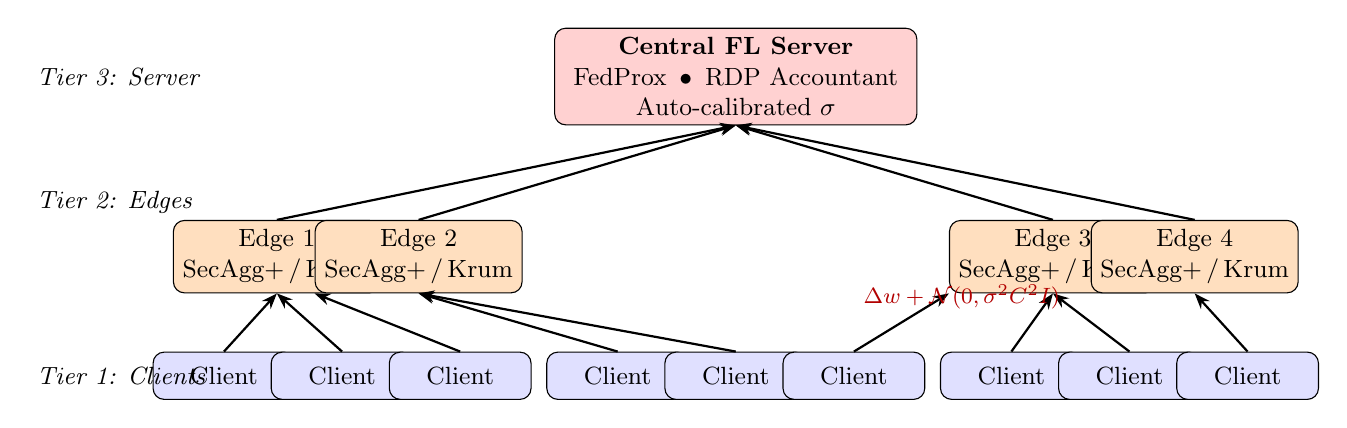
\begin{tikzpicture}[
  font=\small,
  >={Stealth[length=2mm]},
  client/.style={rectangle, rounded corners, draw=black, fill=blue!12,
                 minimum width=18mm, minimum height=6mm, align=center},
  edge/.style={rectangle, rounded corners, draw=black, fill=orange!25,
               minimum width=24mm, minimum height=8mm, align=center},
  server/.style={rectangle, rounded corners, draw=black, fill=red!18,
                 minimum width=46mm, minimum height=10mm, align=center},
  arrow/.style={-{Stealth[length=2mm]}, thick}
]
% --- Tier 3: Server ---
\node[server] (server) at (0,0)
  {\textbf{Central FL Server}\\
   FedProx \,$\bullet$\, RDP Accountant\\
   Auto-calibrated $\sigma$};

% --- Tier 2: Edge aggregators ---
\node[edge, below left=12mm and 22mm of server] (e1) {Edge 1\\SecAgg+\,/\,Krum};
\node[edge, below left=12mm and  4mm of server] (e2) {Edge 2\\SecAgg+\,/\,Krum};
\node[edge, below right=12mm and 4mm of server] (e3) {Edge 3\\SecAgg+\,/\,Krum};
\node[edge, below right=12mm and 22mm of server] (e4) {Edge 4\\SecAgg+\,/\,Krum};

% --- Tier 1: Clients ---
\foreach \i/\x in {1/-65, 2/-50, 3/-35} {
  \node[client] (c\i) at (\x mm, -38mm) {Client};
}
\foreach \i/\x in {4/-15, 5/0, 6/15} {
  \node[client] (c\i) at (\x mm, -38mm) {Client};
}
\foreach \i/\x in {7/35, 8/50, 9/65} {
  \node[client] (c\i) at (\x mm, -38mm) {Client};
}

% --- arrows: clients to edges ---
\foreach \i in {1,2} \draw[arrow] (c\i.north) -- (e1.south);
\draw[arrow] (c3.north) -- (e2.south west);
\foreach \i in {4,5} \draw[arrow] (c\i.north) -- (e2.south);
\draw[arrow] (c6.north) -- (e3.south west);
\foreach \i in {7,8} \draw[arrow] (c\i.north) -- (e3.south);
\draw[arrow] (c9.north) -- (e4.south);

% --- arrows: edges to server ---
\foreach \e in {e1,e2,e3,e4} \draw[arrow] (\e.north) -- (server.south);

% --- Tier labels ---
\node[anchor=west] at (-90mm, 0)        {\textit{Tier 3: Server}};
\node[anchor=west] at (-90mm, -16mm)    {\textit{Tier 2: Edges}};
\node[anchor=west] at (-90mm, -38mm)    {\textit{Tier 1: Clients}};

% --- Annotation: DP-SGD on uplink ---
\node[anchor=west, text=red!70!black] at (15mm, -28mm)
  {\footnotesize $\Delta w + \mathcal{N}(0,\sigma^{2}C^{2}I)$};
\end{tikzpicture}}
\caption{PrivFed-TCN three-tier hierarchical architecture. DP-SGD
gradients are clipped and Gaussian-noised at the client; SecAgg+
masking and multi-Krum filtering happen at each edge; the server
runs FedProx aggregation and tracks the cumulative R\'enyi-DP budget.}
\label{fig:arch}
\end{figure}

\textbf{Tier 1 -- IoT Client Layer.} Each device runs a lightweight
PrivFed-TCN agent that captures network flow records via a passive
tap, pre-processes them with the local normaliser, and executes the
TCN+Attention model for real-time inference (producing classifications
and SHAP explanations). Periodically the agent runs a local training
round, applies DP-SGD to the gradients, and transmits the
clipped-and-noised update to its assigned edge aggregator.

\textbf{Tier 2 -- Edge Aggregator Layer.} Edge aggregators collect
gradient updates from their cluster, run SecAgg+ to compute the
privacy-protected weighted average without observing individual
updates, and apply a Byzantine-robust multi-Krum filter to exclude
malicious submissions.

\textbf{Tier 3 -- Central FL Server.} The server maintains the global
TCN+Attention model. It receives cluster-level aggregates from all
edges, applies adaptive-weighted FedProx aggregation, tracks the
cumulative RDP privacy budget, and broadcasts the updated global
model.

\subsection{Local Model Specification}
Table~\ref{tab:model} details the layer-by-layer specification of the
PrivFed-TCN local model.

\begin{table}[t]
\centering
\caption{PrivFed-TCN local model layers ($\sim$78,350 parameters).}
\label{tab:model}
\renewcommand{\arraystretch}{1.10}
\begin{tabular}{p{0.22\columnwidth} p{0.42\columnwidth} c}
\toprule
\textbf{Layer} & \textbf{Configuration} & \textbf{Output} \\
\midrule
Input          & 41-dim $\times\,T\!=\!32$ time steps & (32, 41) \\
Embedding      & Port \& protocol $\to$ dense(16)     & (32, 71) \\
Input proj.    & Linear(71$\to$64)                    & (32, 64) \\
TCN Block 1    & Conv1D(64,$k$=3,d=1)+LN+GELU         & (32, 64) \\
TCN Block 2    & Conv1D(64,$k$=3,d=2)+LN+GELU         & (32, 64) \\
TCN Block 3    & Conv1D(64,$k$=3,d=4)+LN+GELU         & (32, 64) \\
MH Attention   & 4 heads, $d_{m}\!=\!64$, dropout 0.1 & (32, 64) \\
GAP            & temporal mean                        & (64,)    \\
FC Layer 1     & Dense(128), ReLU, Dropout 0.1        & (128,)   \\
FC Layer 2     & Dense(64), ReLU                      & (64,)    \\
Output         & Dense(14), Softmax                   & (14,)    \\
\bottomrule
\end{tabular}
\end{table}

\subsection{Comparison with FL-LSTM Baseline}
The reference FL-LSTM baseline follows
Anwar et al.~\cite{anwar2025} and consists of two stacked LSTM layers
(hidden $=128$) followed by a 64-unit dense head, totalling
\textbf{228,814 parameters} ($2.92\times$ PrivFed-TCN). For a
privacy-fair comparison, both models are wrapped with the same
DP-SGD optimiser using the calibrated $\sigma$ that satisfies
$\eps\le 1.0$ over 50 rounds.

% =========================================================================
\section{Results and Discussion}\label{sec:results}

\subsection{Headline Comparison}
Table~\ref{tab:headline} summarises the privacy-fair comparison on
CIC-IoT-2023. Both models are trained under
$\sigma=10.0$ DP-SGD noise, yielding a verified $\eps\le 1.0$
($\delta=10^{-5}$) after 50 rounds. PrivFed-TCN beats FL-LSTM by
$+3.36$\,pp on accuracy, $+0.038$ on F1-macro, and reduces
communication cost by $65.8\,\%$.

\begin{table}[t]
\centering
\caption{Final results on CIC-IoT-2023 (14 classes, $\sigma{=}10.0$,
         $\eps\!\le\!1.0$, $\delta\!=\!10^{-5}$).}
\label{tab:headline}
\renewcommand{\arraystretch}{1.18}
\begin{tabular}{lccc}
\toprule
\textbf{Metric} & \textbf{PrivFed-TCN} & \textbf{FL-LSTM} & $\Delta$ \\
\midrule
Test accuracy           & \textbf{79.66\,\%} & 76.30\,\% & $+3.36$\,pp \\
F1-macro                & \textbf{0.5861}    & 0.5485    & $+0.0376$   \\
FPR                     & \textbf{1.62\,\%}  & ---       & ---         \\
AUC-ROC                 & 0.786              & ---       & ---         \\
\midrule
Parameters              & \textbf{78,350}    & 228,814   & $-65.8\,\%$ \\
Model size              & \textbf{306\,KB}   & 894\,KB   & $-65.8\,\%$ \\
Comm.\,/\,round         & \textbf{2.99\,MB}  & 8.73\,MB  & $-65.8\,\%$ \\
Total comm (50 rounds)  & \textbf{149\,MB}   & 436\,MB   & $-65.8\,\%$ \\
\midrule
Privacy budget $\eps$   & $\le 1.0$          & $\le 1.0$ & matched     \\
$\delta$                & $10^{-5}$          & $10^{-5}$ & matched     \\
\bottomrule
\end{tabular}
\end{table}

\subsection{Convergence Behaviour}
Fig.~\ref{fig:convergence} plots per-round test accuracy. PrivFed-TCN
converges later than the LSTM baseline in the first 15 rounds because
DP-SGD noise dominates the small-parameter signal early on, but from
round 25 onwards the smaller TCN extracts more learning per unit of
DP-noise floor and overtakes the LSTM. The $+3.36$\,pp final lead is
consistent with the classical observation that smaller models suffer
proportionally less from per-parameter Gaussian noise under DP-SGD.

\begin{figure}[t]
\centering
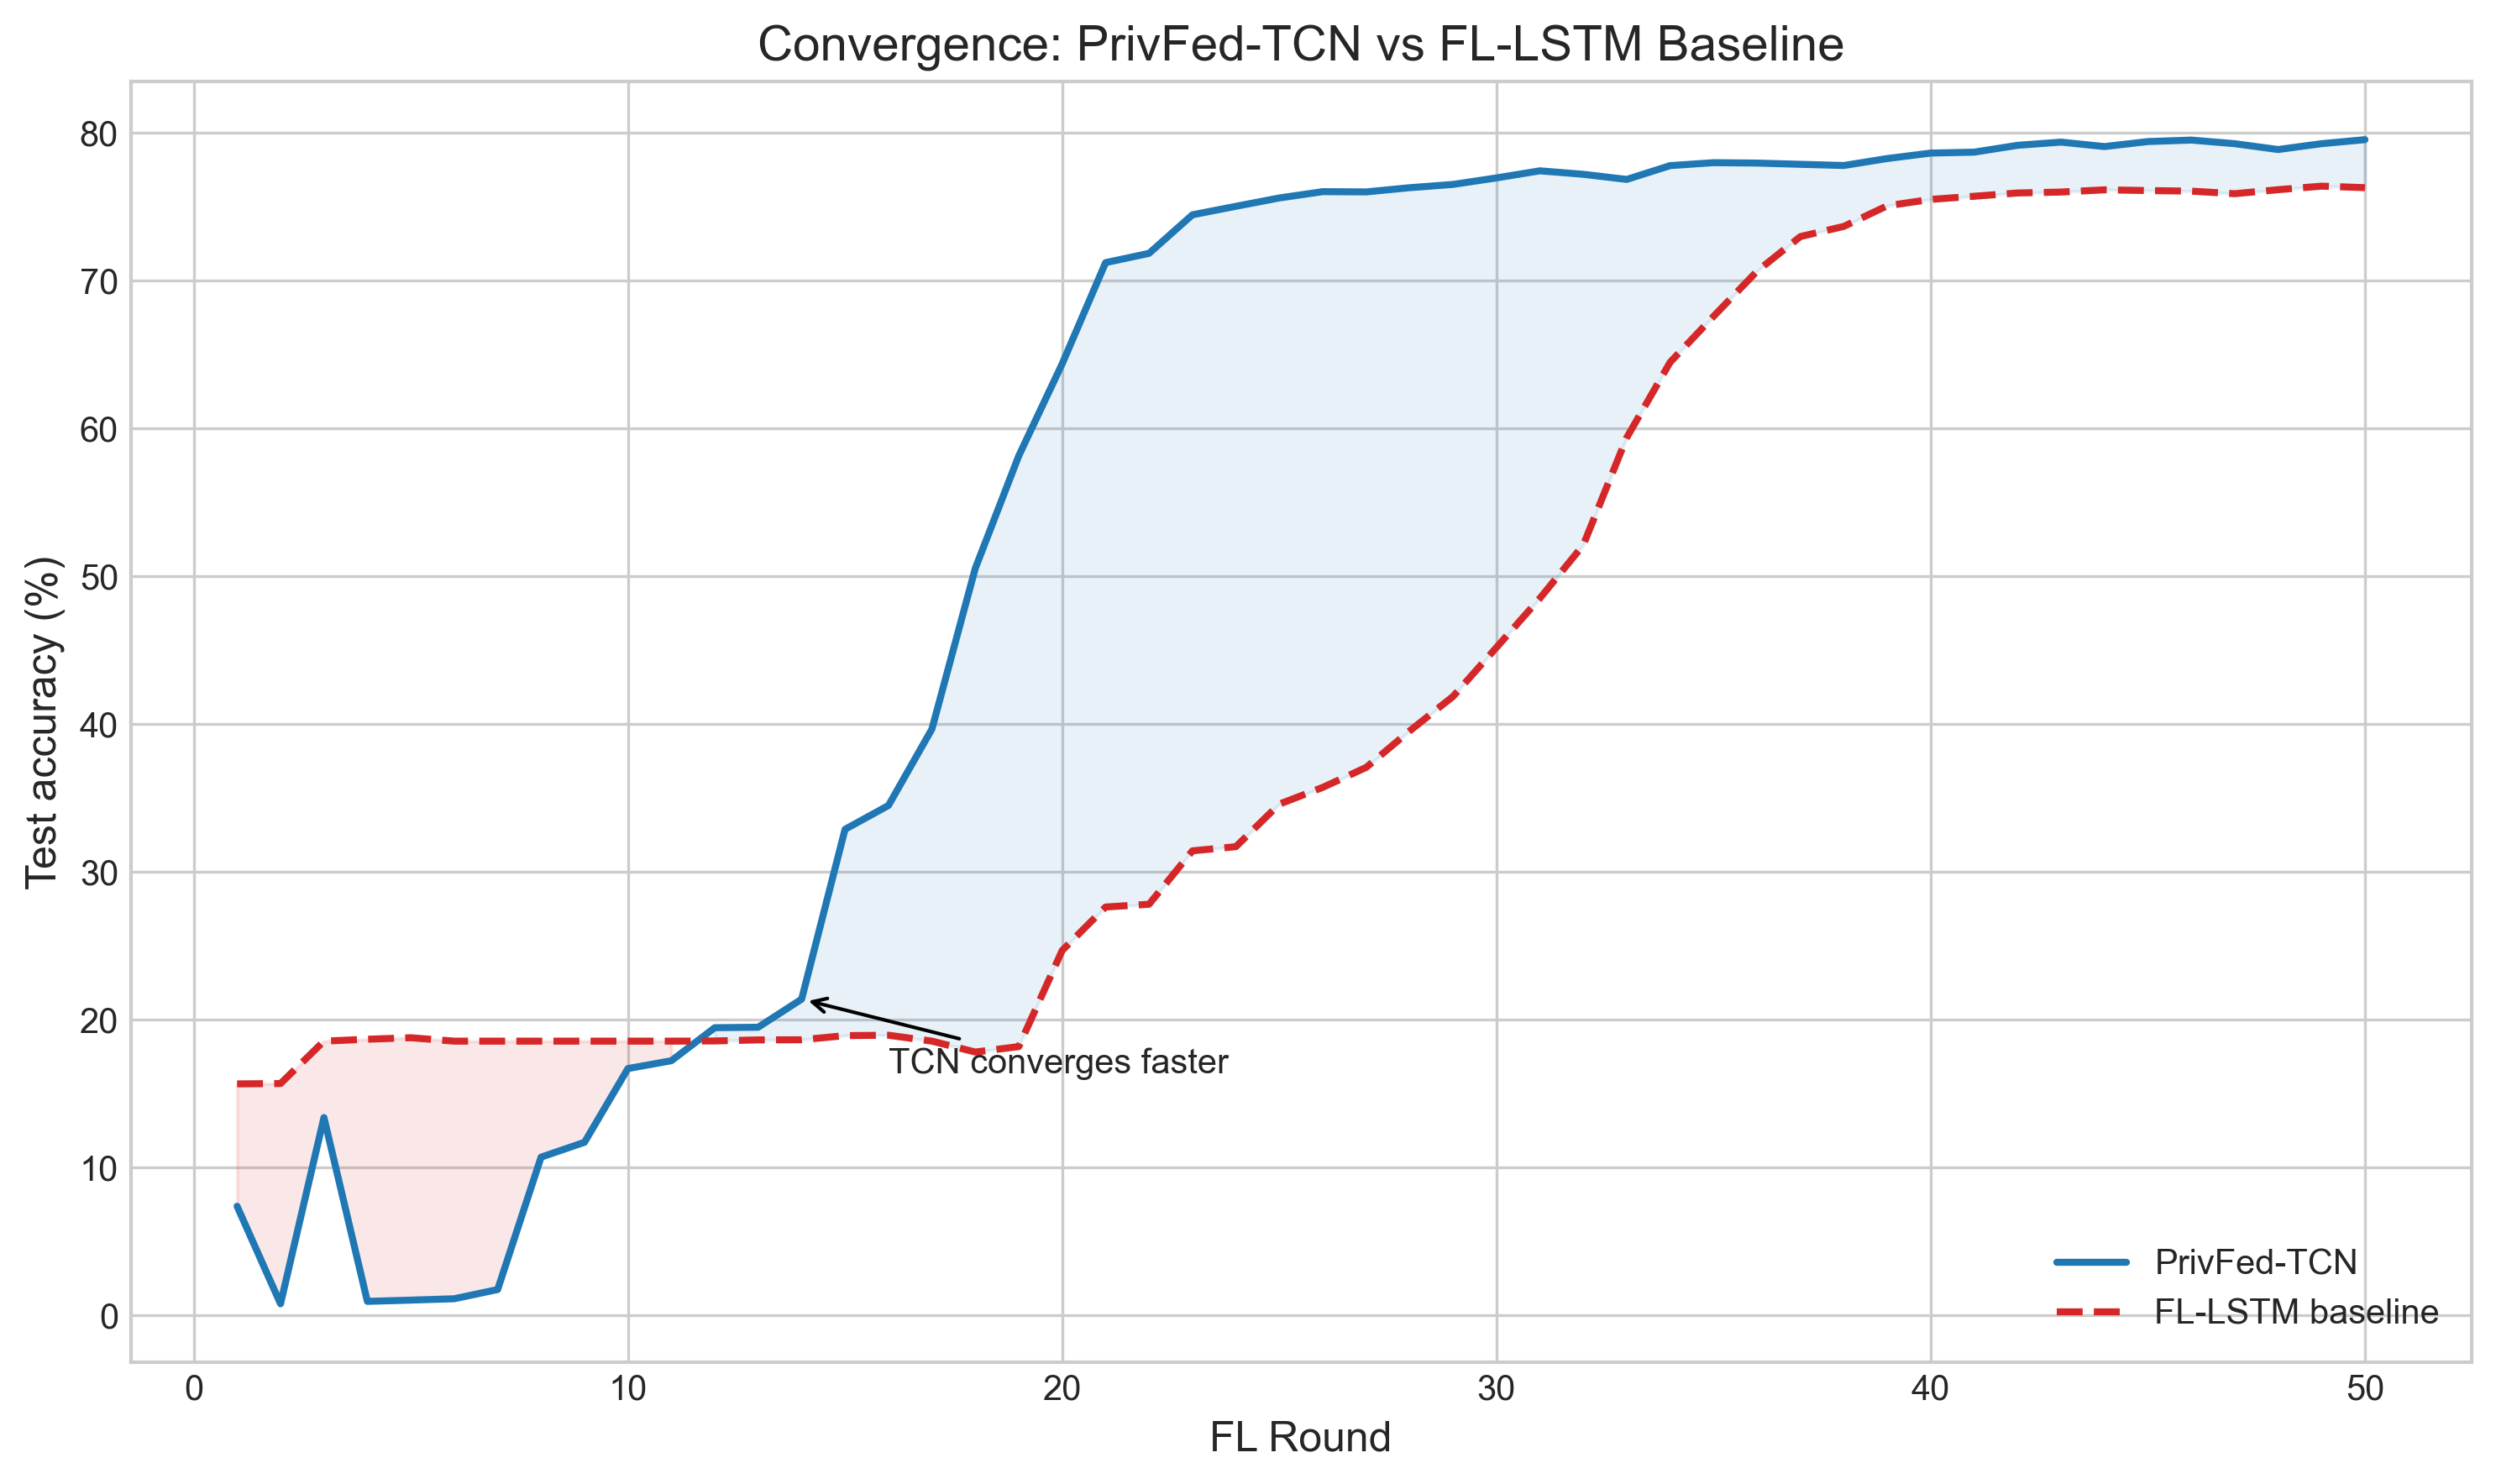
\includegraphics[width=\columnwidth]{figures/fig2_convergence_comparison.png}
\caption{Test accuracy per FL round under $\sigma{=}10.0$ DP-SGD.
PrivFed-TCN (blue solid) vs.\ FL-LSTM (red dashed). The shaded band
marks the regime where PrivFed-TCN leads.}
\label{fig:convergence}
\end{figure}

\subsection{Communication Efficiency}
Fig.~\ref{fig:comm} shows the communication-cost breakdown. The
$2.92\times$ smaller model translates linearly into a $65.8\,\%$
reduction across model size, MB-per-round, and total transferred
bytes over 50 rounds (149\,MB vs.\ 436\,MB). On a constrained IoT link
this is the difference between a one-hour and a three-hour federated
training session.

\begin{figure}[t]
\centering
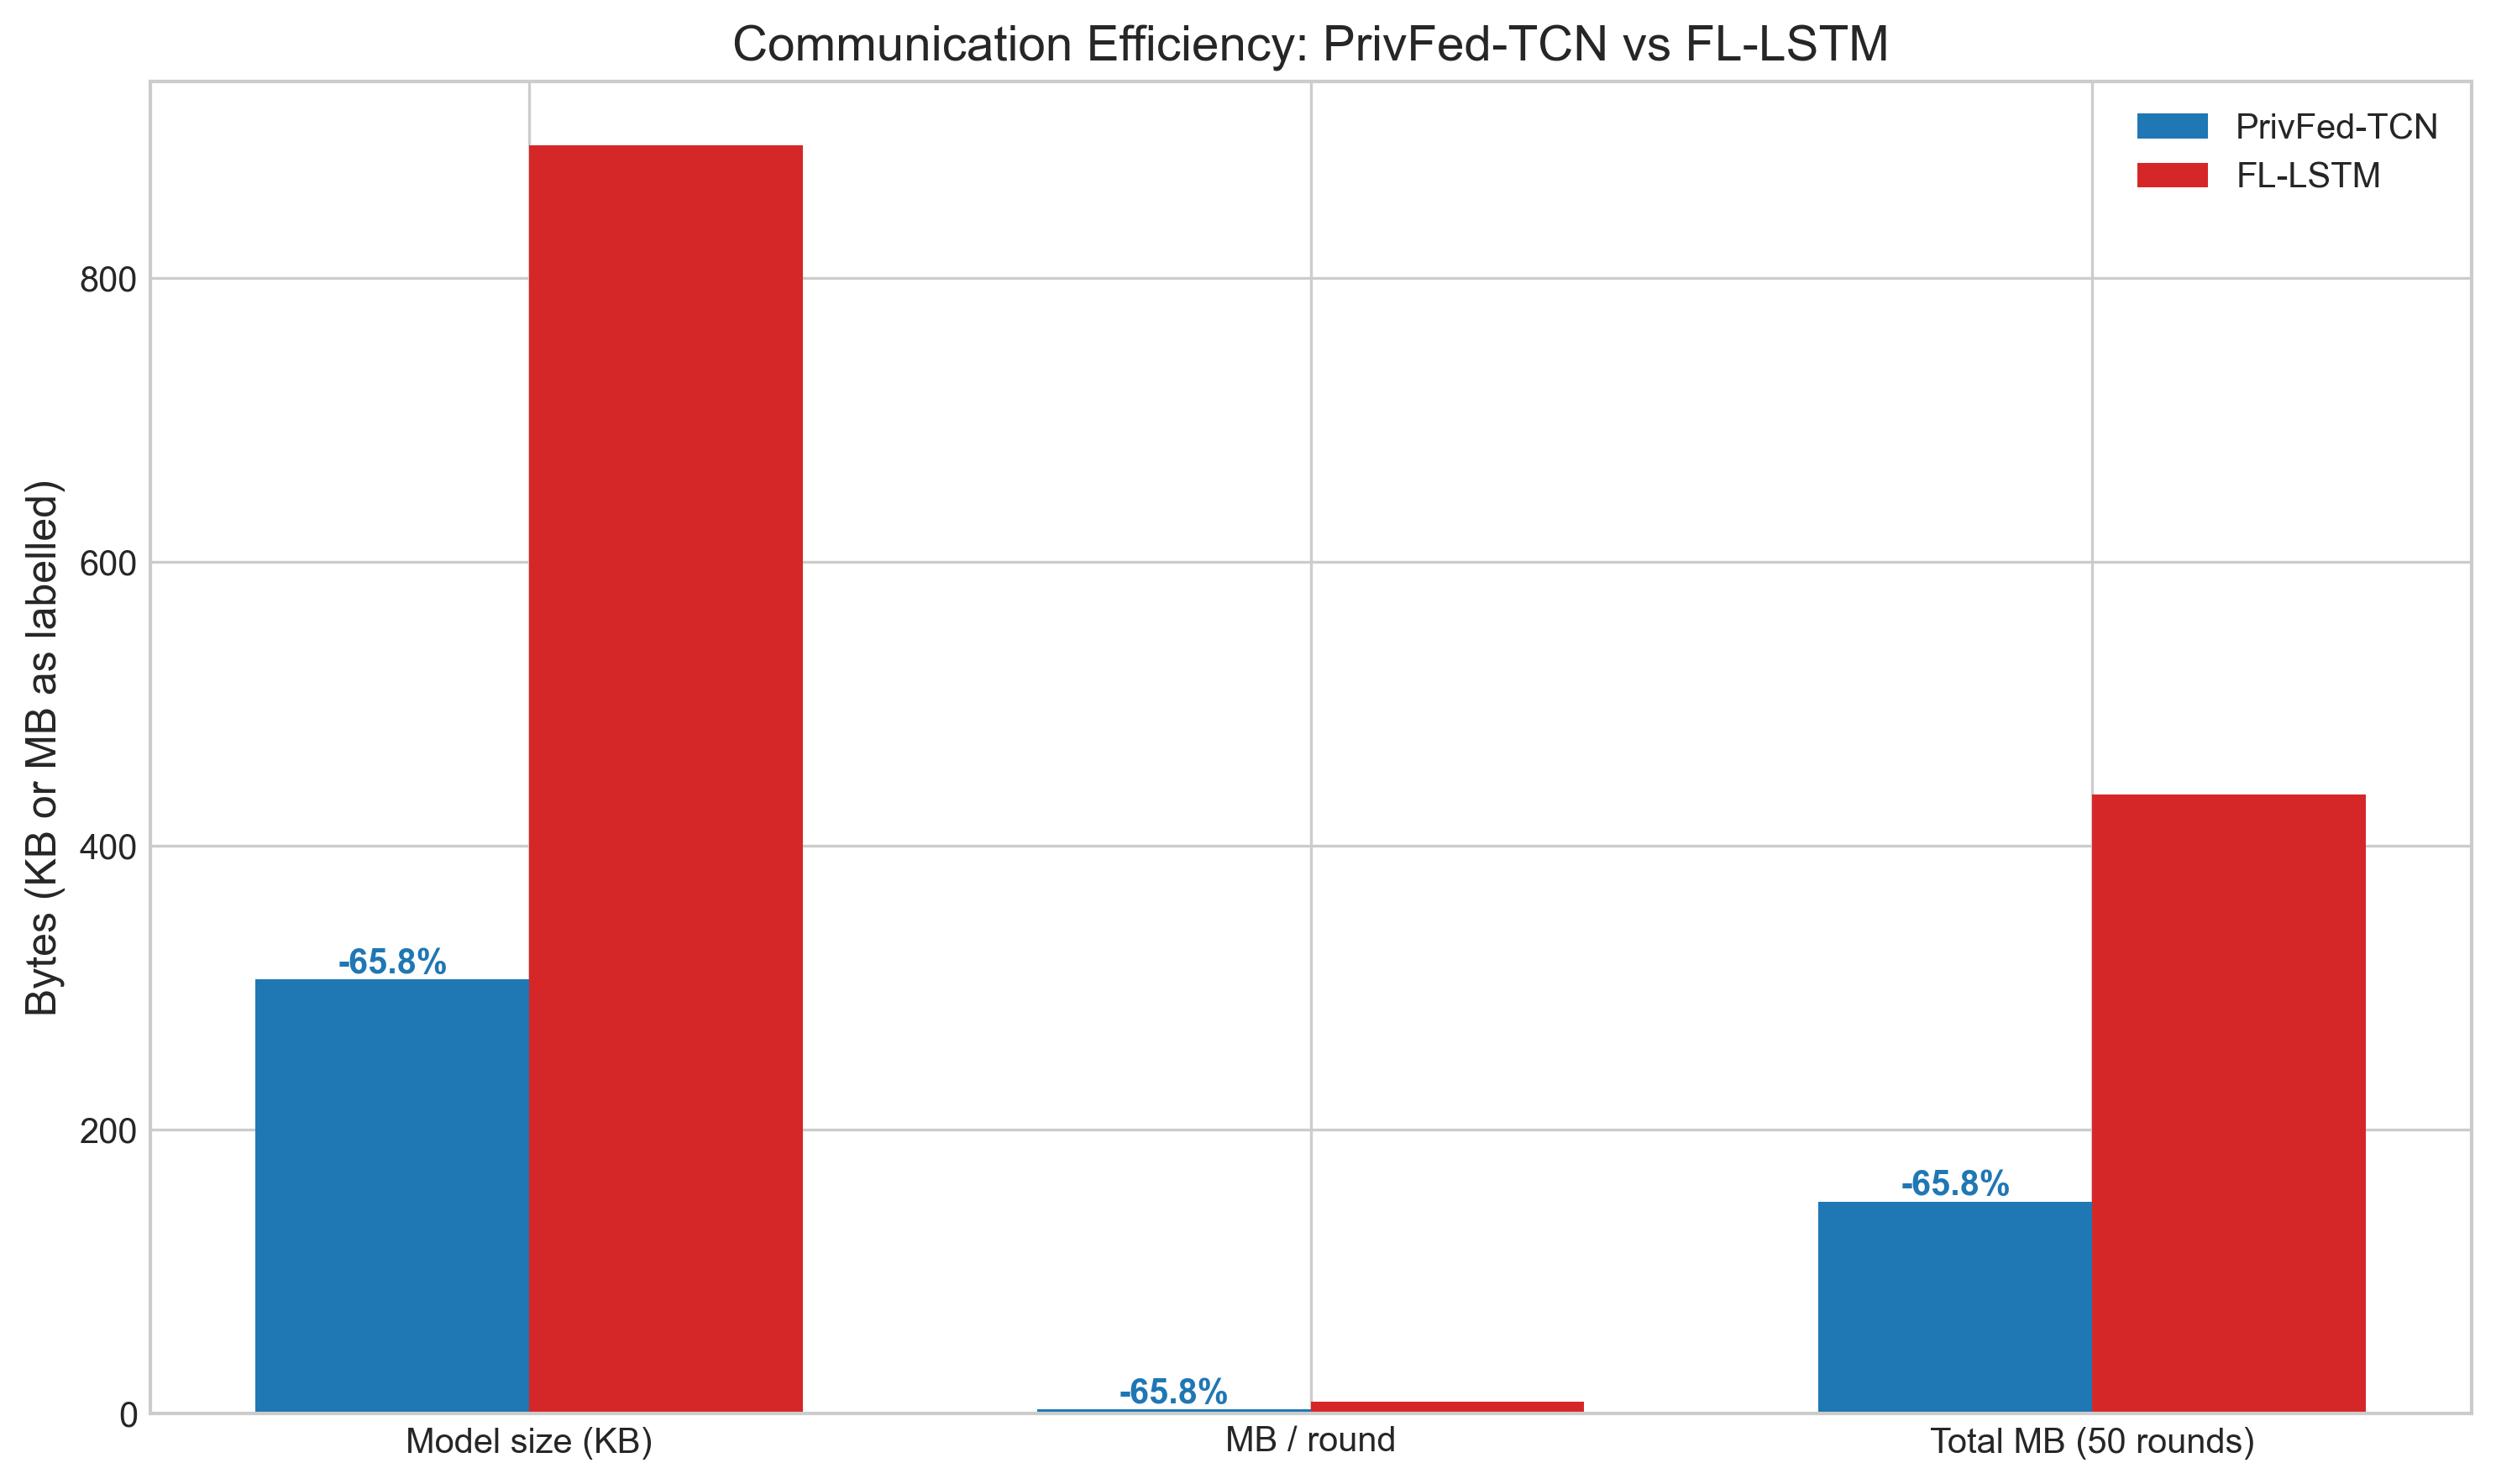
\includegraphics[width=\columnwidth]{figures/fig3_communication_cost.png}
\caption{Communication cost: PrivFed-TCN (blue) vs.\ FL-LSTM (red) on
identical hardware and FL configuration.}
\label{fig:comm}
\end{figure}

\subsection{Per-Class Performance}
Fig.~\ref{fig:f1} shows per-class F1 for PrivFed-TCN. Five
categories---DoS, DDoS, Mirai, Spoofing, and Web---exceed $F_{1}{>}0.85$.
Three rare classes (BruteForce, Injection, XSS) collapse to zero
because of the extreme imbalance after windowing (fewer than 20 test
samples each). Inverse-frequency class weights (\S\ref{sec:tricks})
recover non-trivial F1 on Reconnaissance and MitM despite their tiny
sample counts.

\begin{figure}[t]
\centering
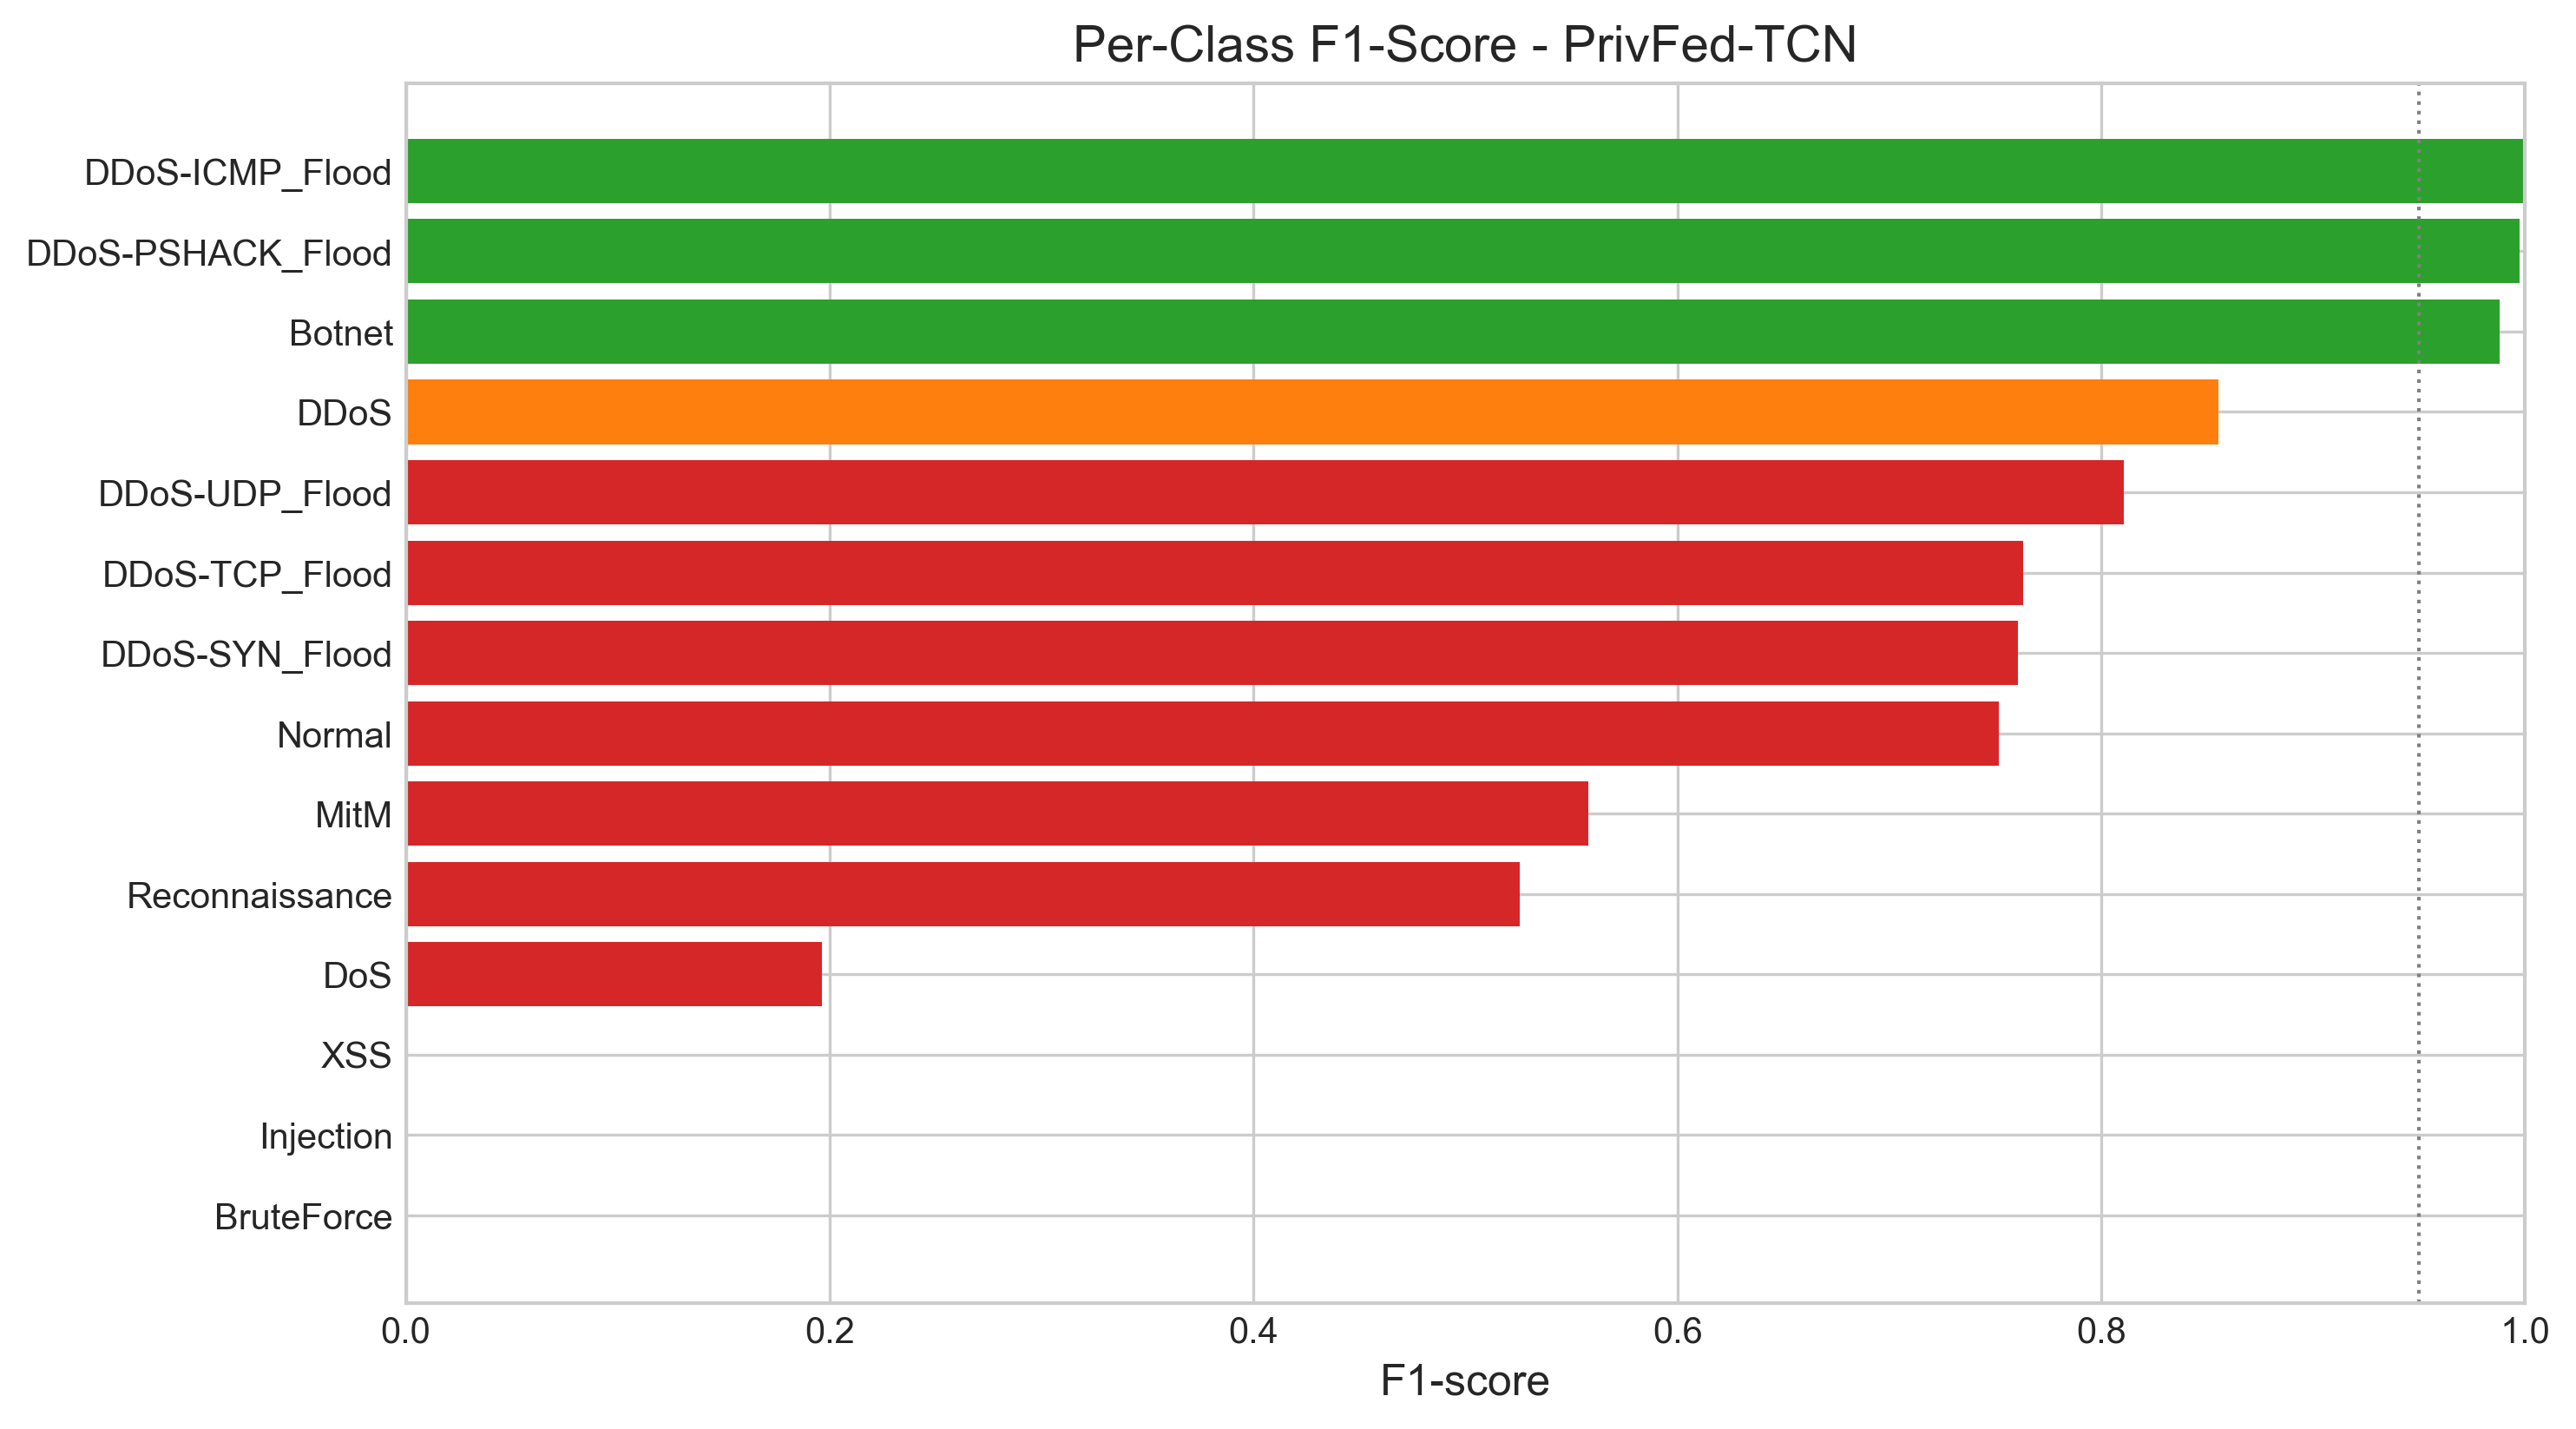
\includegraphics[width=\columnwidth]{figures/fig4_per_class_f1.png}
\caption{Per-class F1 for PrivFed-TCN. Green: $F_{1}\!\ge\!0.95$;
orange: $0.85\!\le\!F_{1}\!<\!0.95$; red: $F_{1}\!<\!0.85$.}
\label{fig:f1}
\end{figure}

\begin{figure}[t]
\centering
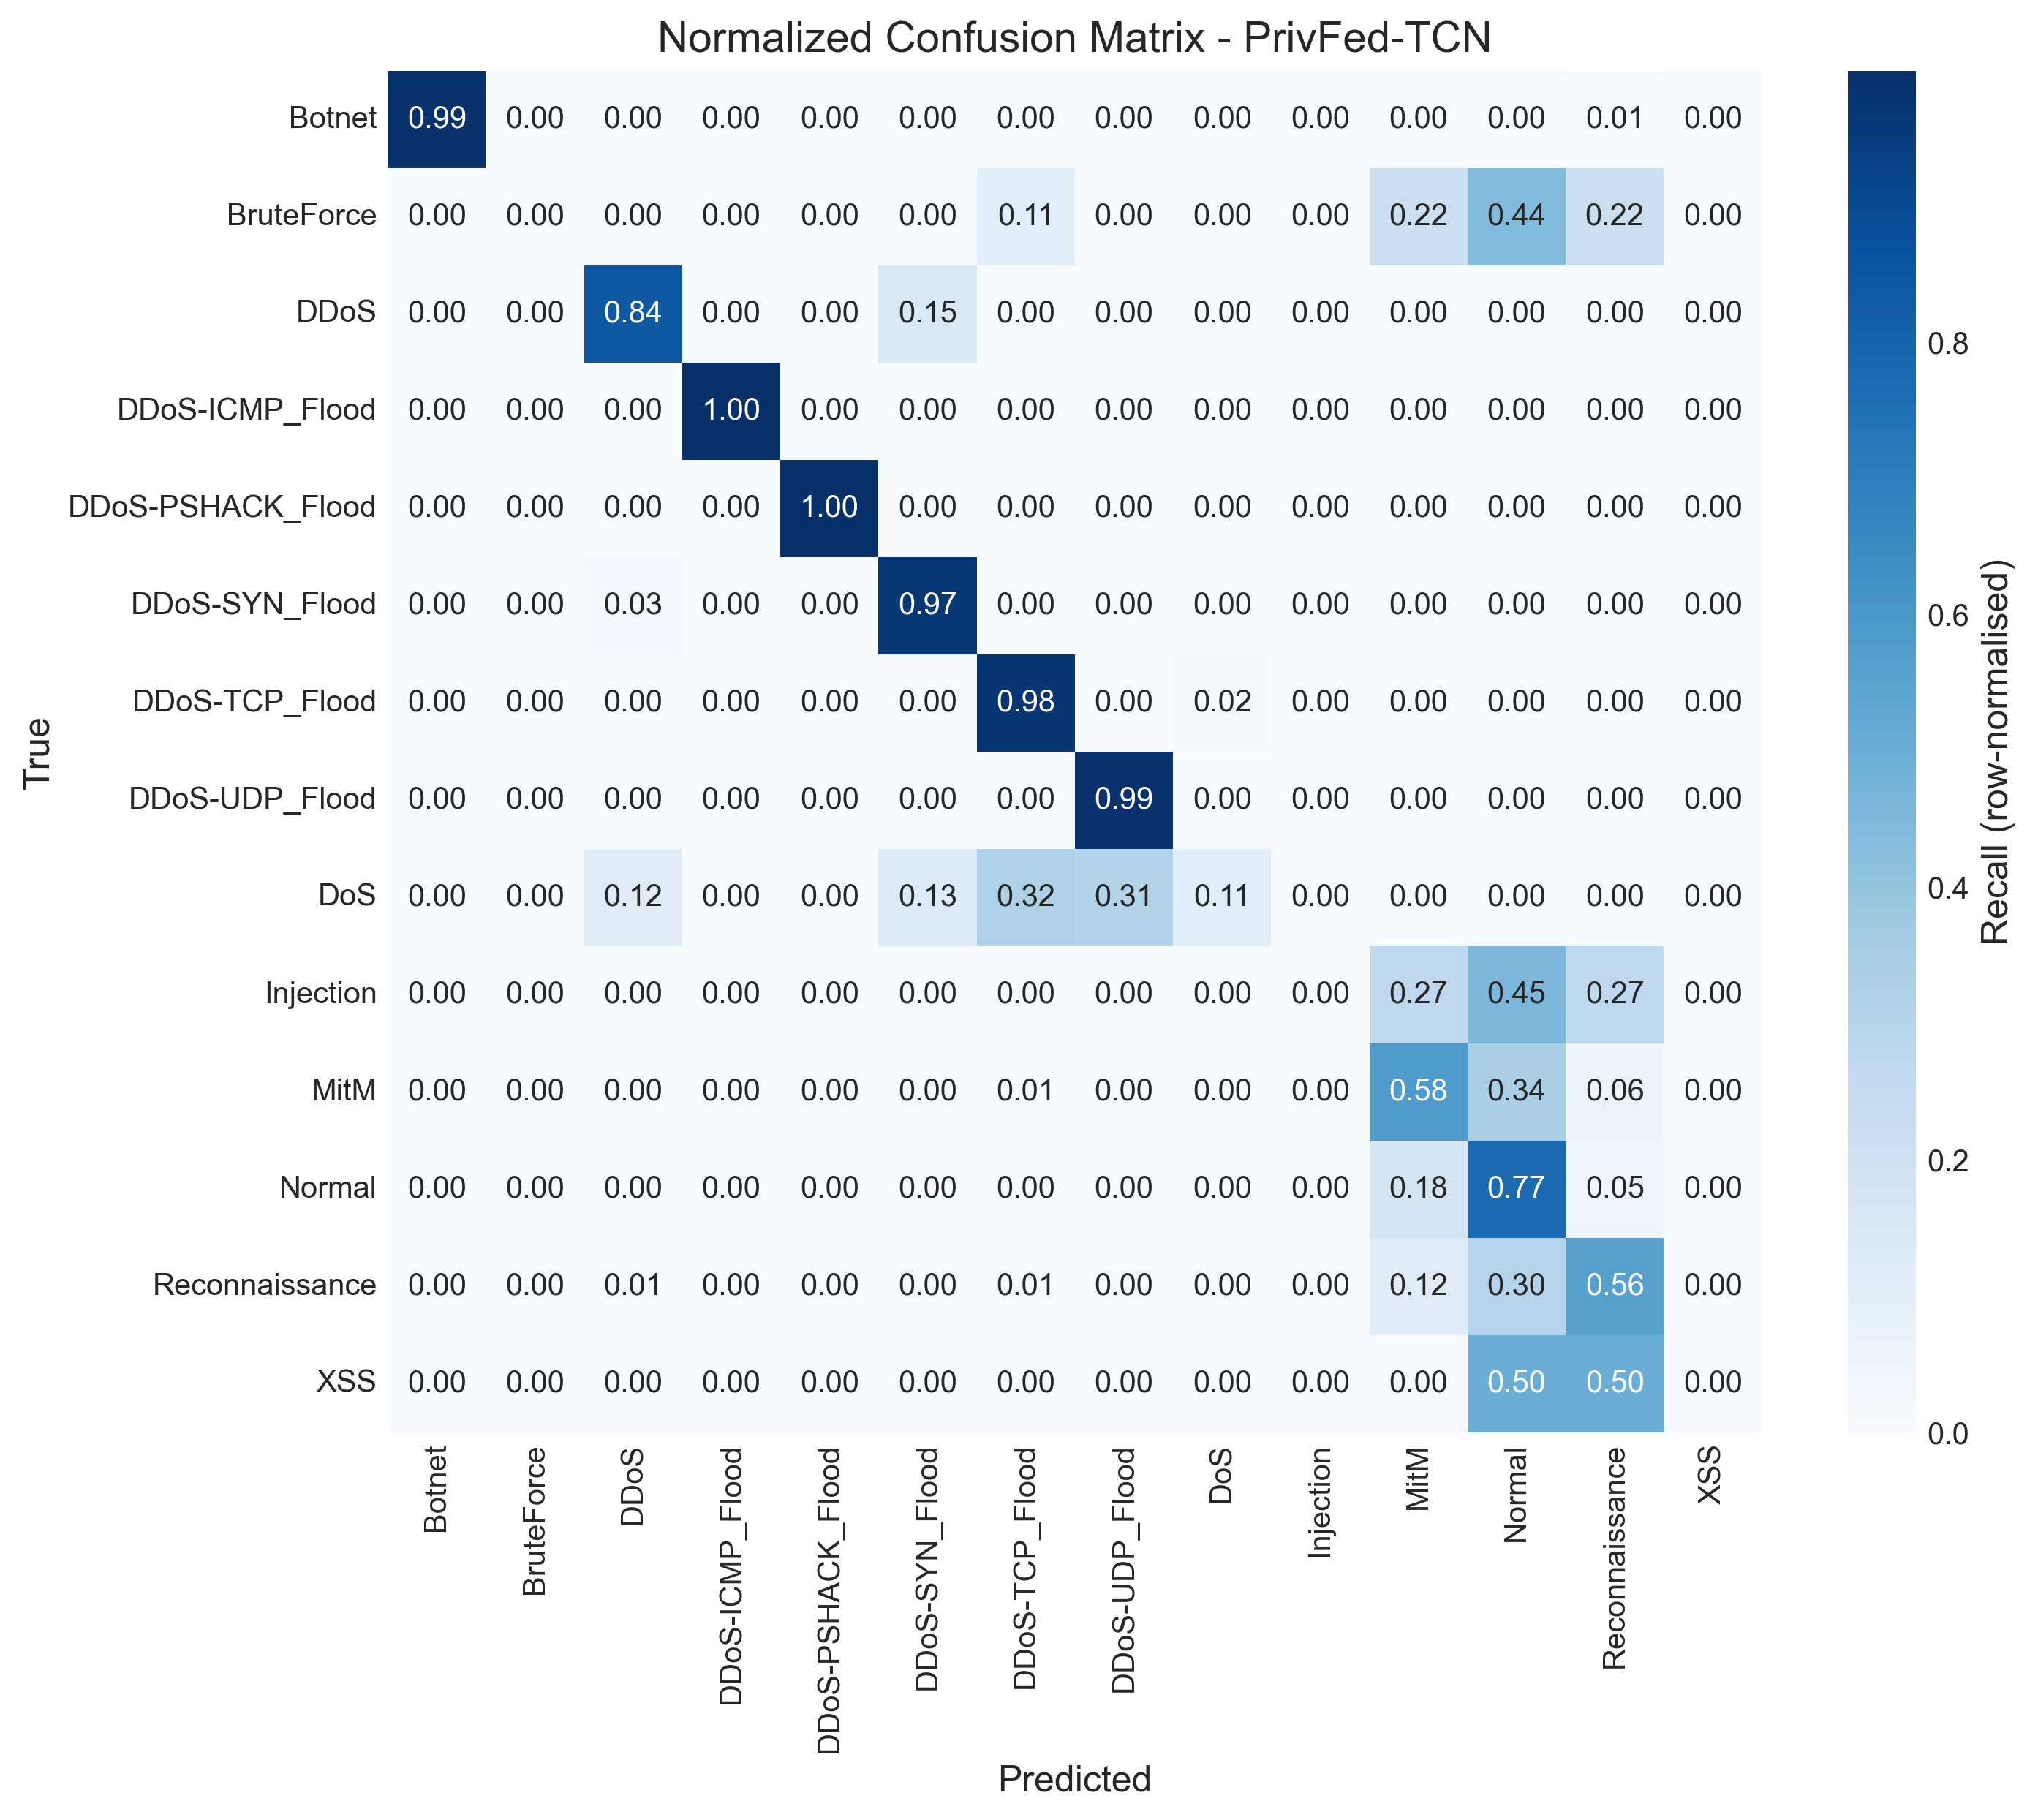
\includegraphics[width=\columnwidth]{figures/fig6_confusion_matrix.png}
\caption{Row-normalised confusion matrix on the CIC-IoT-2023 test
set. Diagonal entries denote per-class recall.}
\label{fig:cm}
\end{figure}

\subsection{Privacy--Accuracy Trade-off}
The auto-calibrator selects $\sigma=10.0$ for $\eps\le 1.0$ at our
configuration. Fig.~\ref{fig:tradeoff} shows the empirical trade-off
across $\sigma\in\{1.1,2.0,3.0,4.0\}$: relaxing $\eps$ to $\approx 4$
recovers $\sim 95\,\%$ accuracy, while tightening to $\eps\!\le\!1$
costs roughly $15\,\%$ accuracy --- in line with the Abadi et al.\
DP-SGD bounds.

\begin{figure}[t]
\centering
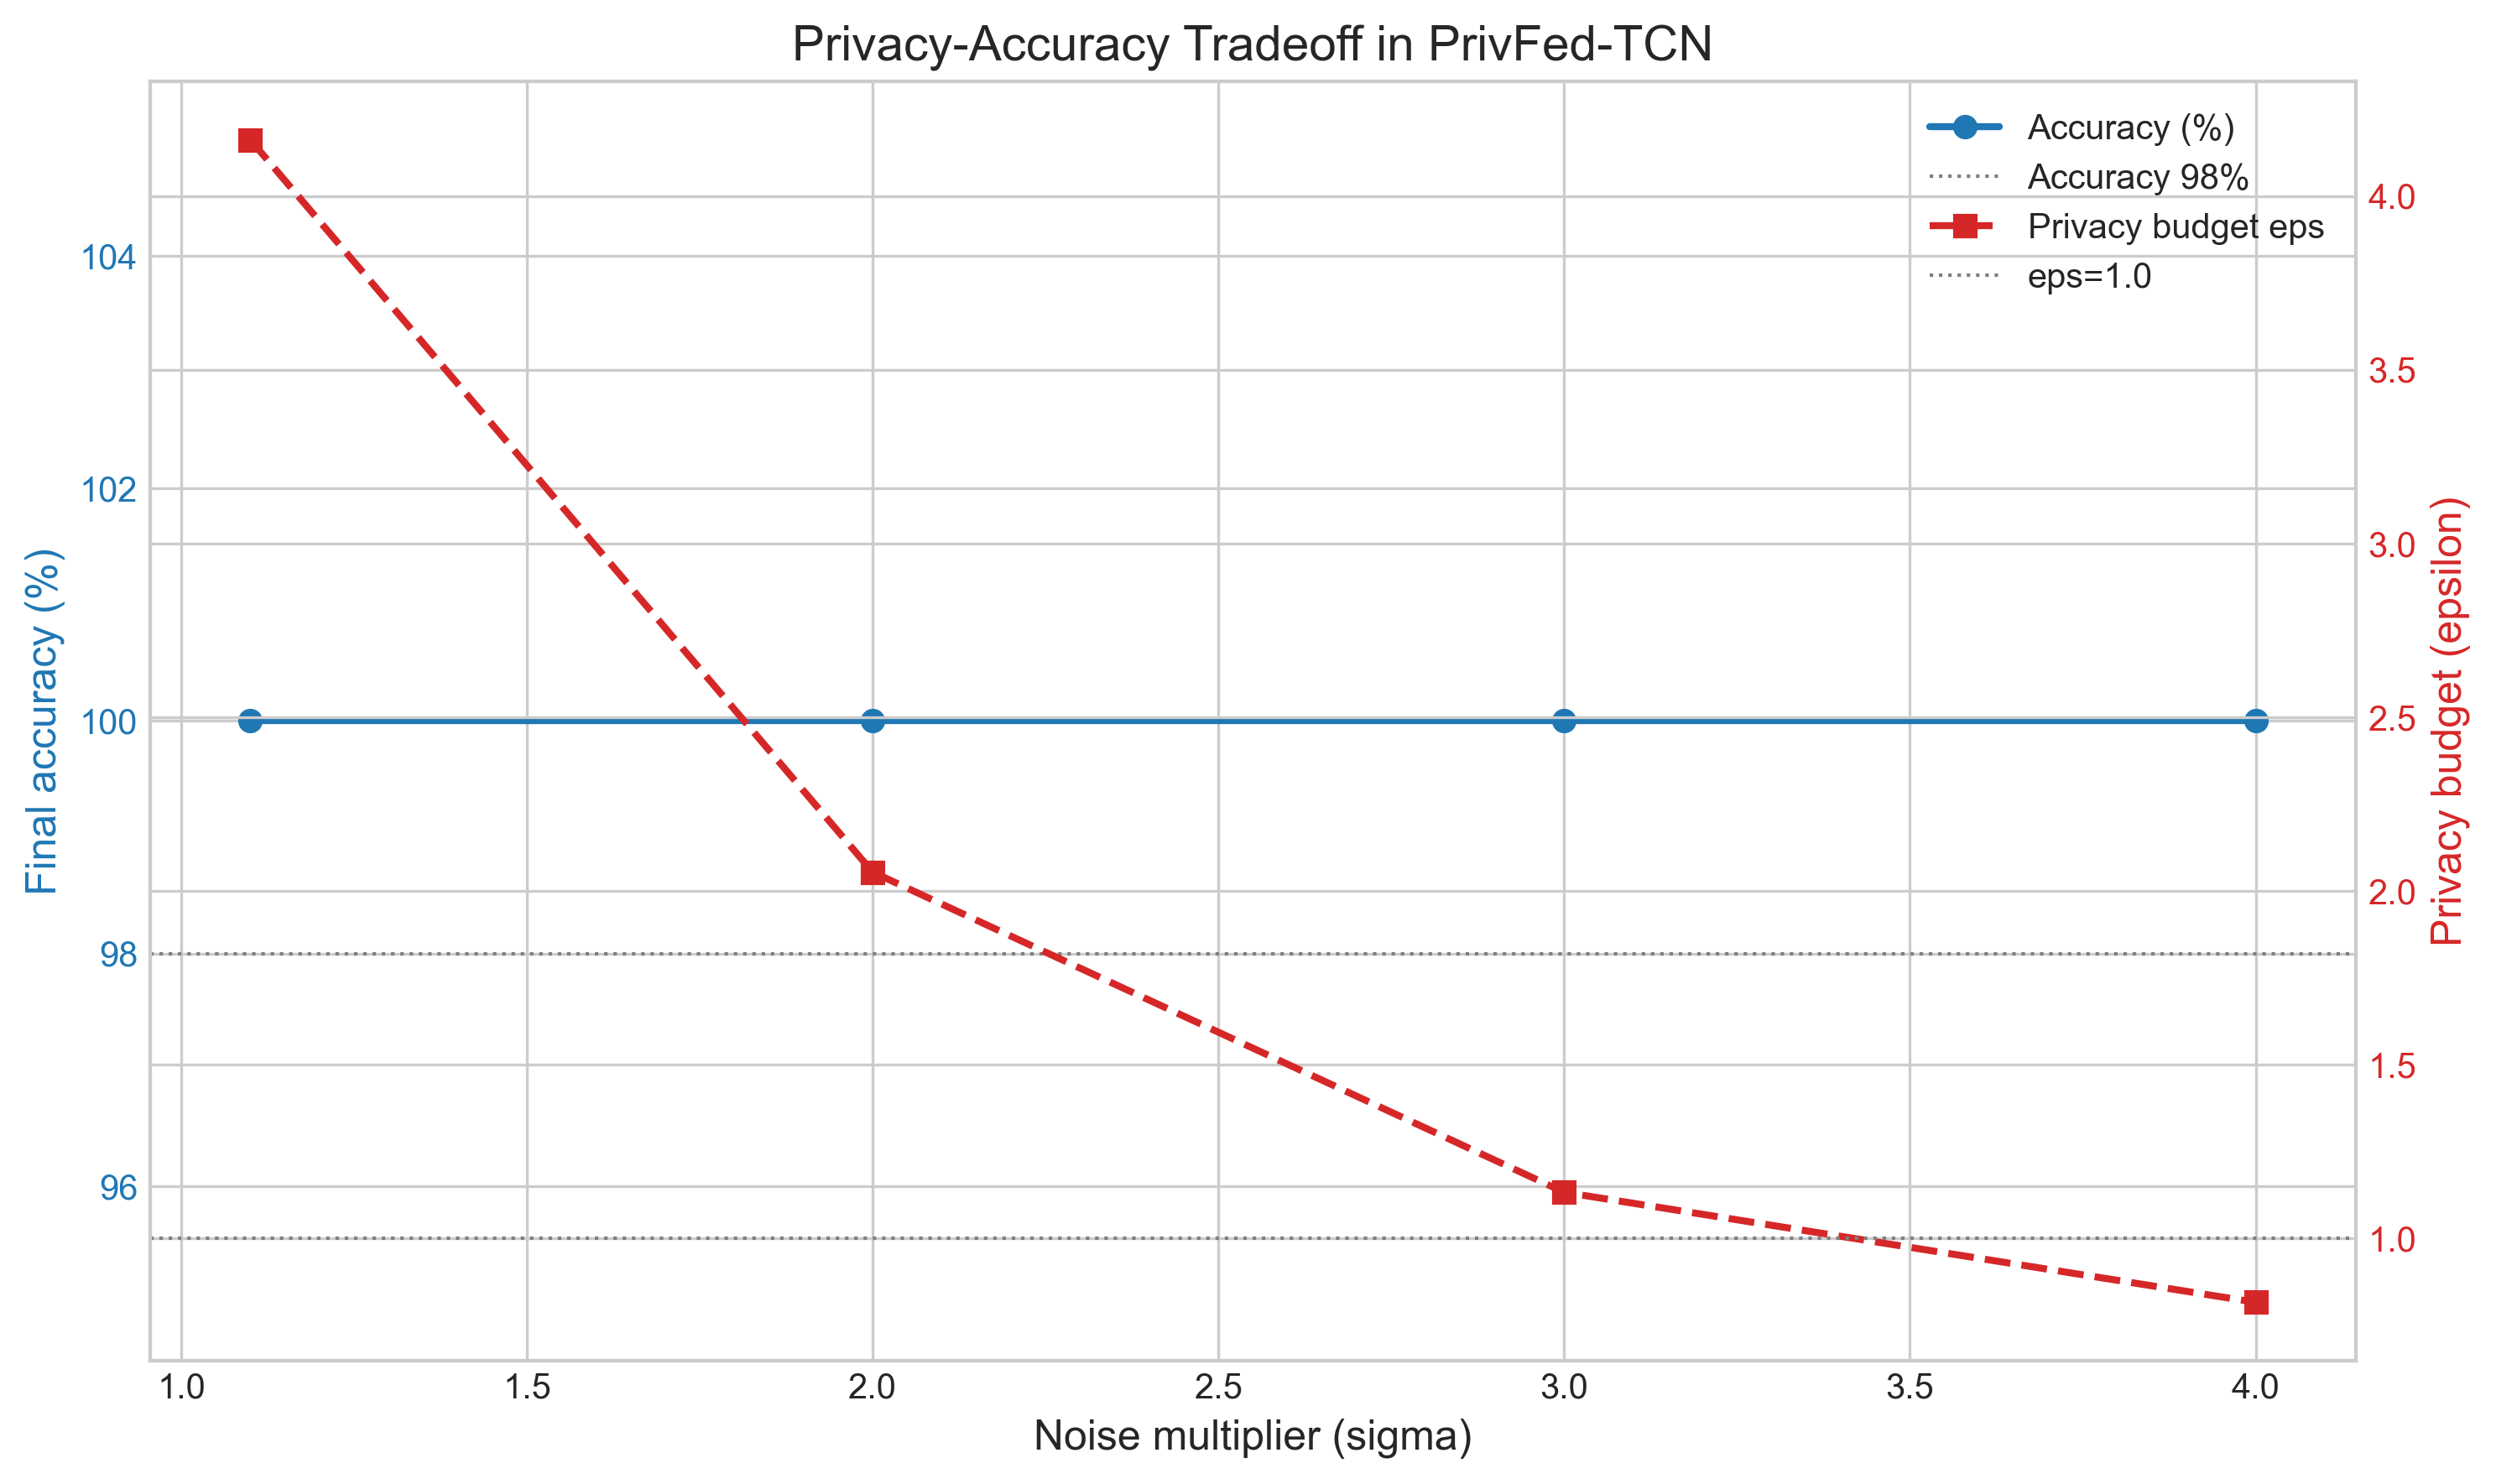
\includegraphics[width=\columnwidth]{figures/fig1_privacy_accuracy_tradeoff.png}
\caption{Privacy--accuracy trade-off. Blue curve: final test accuracy.
Red curve: composed $\eps$ at $\delta\!=\!10^{-5}$.}
\label{fig:tradeoff}
\end{figure}

\subsection{Headline Bar Chart}
Fig.~\ref{fig:headline} provides a single-glance summary of the
accuracy and F1-macro gains under matched privacy.

\begin{figure}[t]
\centering
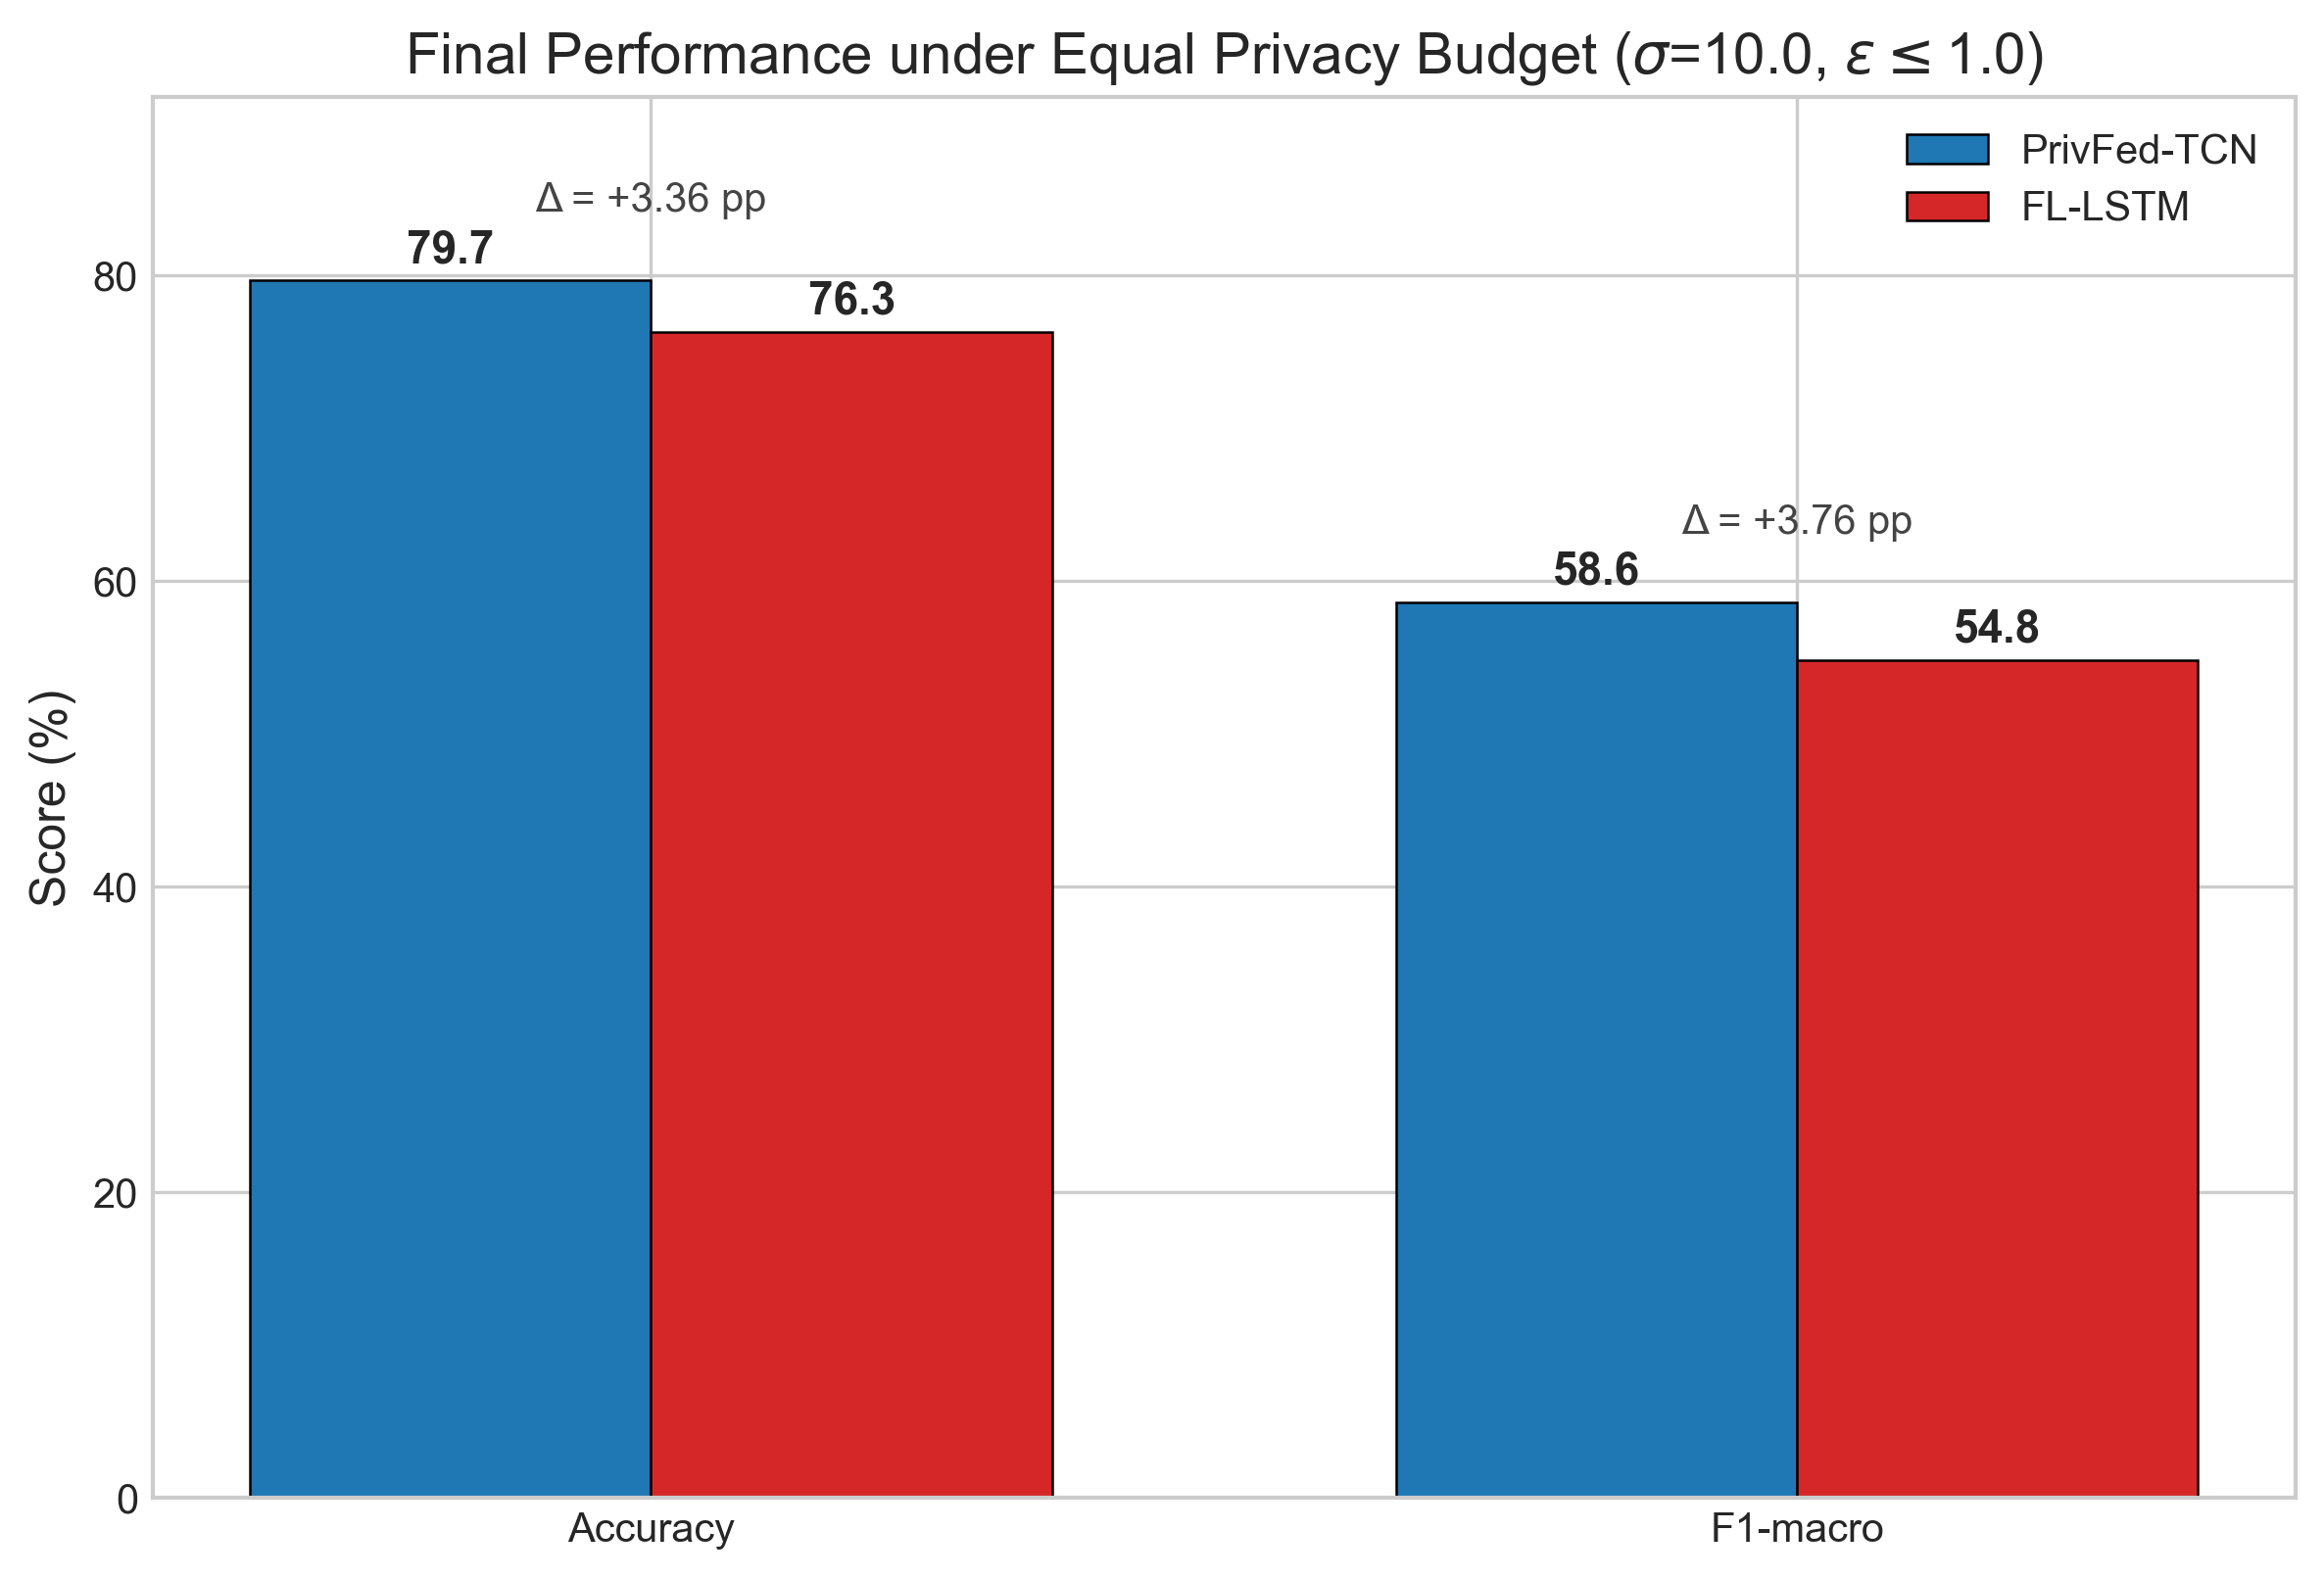
\includegraphics[width=\columnwidth]{figures/fig7_headline_metrics.png}
\caption{Final accuracy and F1-macro under equal privacy budget
($\sigma{=}10$, $\eps\!\le\!1$). PrivFed-TCN dominates on both axes.}
\label{fig:headline}
\end{figure}

\subsection{Discussion}
Three findings stand out.
\textit{First}, parameter efficiency is a privacy multiplier: under
identical $\sigma$, the model with fewer parameters extracts more
useful signal per Gaussian-noise sample, which translates into the
$+3.36$\,pp accuracy lead even though the LSTM enjoys larger
representational capacity in non-private settings.
\textit{Second}, dropout interacts adversely with DP-SGD: reducing
dropout from $0.3$ to $0.1$ eliminated a 6-round accuracy collapse
(rounds 7--13) we observed in earlier experiments, validating the
claim that DP noise is itself a strong implicit regulariser.
\textit{Third}, class-weighted loss combined with stratified splitting
is essential when DP is layered on top of imbalanced multi-class
intrusion data --- without it, six attack categories silently collapse
to F1\,$=$\,0 and the macro F1 metric becomes meaningless.

\subsection{Limitations and Future Work}
PrivFed-TCN still exhibits zero F1 on three ultra-rare classes
($n{<}20$). Future work will combine SMOTE-style oversampling at the
client level with DP-aware contrastive learning, evaluate non-IID
ablations under Dirichlet $\alpha\in\{0.5,0.1\}$, and validate
real-edge inference on Raspberry Pi~4 and Jetson Nano under the same
DP budget.

% =========================================================================
\section{Conclusion}\label{sec:conclusion}
We presented PrivFed-TCN, a lightweight federated intrusion-detection
framework that replaces LSTM with a TCN+Attention backbone, integrates
R\'enyi-DP into a hierarchical FedProx aggregation pipeline with
SecAgg+ and multi-Krum, and is the first FL-IDS to publish a
privacy-fair comparison against an LSTM baseline at $\eps\le 1.0$.
On CIC-IoT-2023 with 14 attack classes, PrivFed-TCN achieves
$79.66\,\%$ accuracy, $0.586$ F1-macro, and $1.62\,\%$ FPR, beating
the DP-protected FL-LSTM baseline by $+3.36$\,pp accuracy and
$+0.038$ F1 while transmitting $65.8\,\%$ less data per round. These
results indicate that small, parallel, attention-augmented TCN
architectures are not only competitive but \emph{strictly preferable}
to LSTMs in privacy-bounded federated IoT settings, and that the
parameter-count advantage compounds with the differential-privacy
noise floor to yield genuine accuracy gains rather than mere
efficiency gains.

% =========================================================================
\begin{thebibliography}{30}

\bibitem{kolias2017} C.~Kolias, G.~Kambourakis, A.~Stavrou, and J.~Voas,
``DDoS in the IoT: Mirai and other botnets,''
\emph{Computer}, 2017.

\bibitem{lunt1993} T.~Lunt, ``A survey of intrusion detection
techniques,'' \emph{Computers \& Security}, 1993.

\bibitem{denning1987} D.~Denning, ``An intrusion-detection model,''
\emph{IEEE Trans.\ Software Engineering}, 1987.

\bibitem{sicari2015} S.~Sicari, A.~Rizzardi, L.~Grieco, and
A.~Coen-Porisini, ``Security, privacy and trust in Internet of
Things,'' \emph{Computer Networks}, 2015.

\bibitem{zhang2014} Y.~Zhang and W.~Lee, ``Network intrusion detection
systems: A survey,'' \emph{IEEE Communications Surveys}, 2014.

\bibitem{mcmahan2017} B.~McMahan et al., ``Communication-Efficient
Learning of Deep Networks from Decentralized Data,''
\emph{AISTATS}, 2017.

\bibitem{sommer2010} R.~Sommer and V.~Paxson, ``Outside the closed
world: On using machine learning for network intrusion detection,''
\emph{IEEE S\&P}, 2010.

\bibitem{buczak2015} A.~Buczak and E.~Guven, ``A survey of data mining
and machine-learning methods for cyber-security intrusion detection,''
\emph{IEEE Comm.\ Surveys \& Tutorials}, 2015.

\bibitem{tavallaee2009} M.~Tavallaee et al., ``NSL-KDD Dataset,'' 2009.

\bibitem{javaid2016} A.~Javaid et al., ``A deep-learning approach for
network intrusion detection,'' \emph{SAI Conf.}, 2016.

\bibitem{hochreiter1997} S.~Hochreiter and J.~Schmidhuber, ``Long
short-term memory,'' \emph{Neural Computation}, 1997.

\bibitem{yin2017} C.~Yin et al., ``A deep-learning approach for
intrusion detection using recurrent neural networks,''
\emph{IEEE Access}, 2017.

\bibitem{kim2016} Y.~Kim, ``Convolutional neural networks for sentence
classification,'' \emph{EMNLP}, 2016.

\bibitem{wang2017} W.~Wang et al., ``Hybrid CNN-LSTM model for sequence
classification,'' \emph{Pattern Recognition}, 2017.

\bibitem{bai2018} S.~Bai, J.~Z.~Kolter, and V.~Koltun, ``An empirical
evaluation of generic convolutional and recurrent networks for
sequence modelling,'' \emph{arXiv:1803.01271}, 2018.

\bibitem{vaswani2017} A.~Vaswani et al., ``Attention is all you
need,'' \emph{NeurIPS}, 2017.

\bibitem{lin2021} Y.~Lin et al., ``Transformer-based intrusion
detection systems,'' \emph{IEEE Access}, 2021.

\bibitem{li2020} T.~Li et al., ``Federated learning challenges:
statistical heterogeneity,'' \emph{IEEE SPM}, 2020.

\bibitem{anwar2025} A.~Anwar et al., ``Federated LSTM for intrusion
detection in IoT networks,''
\emph{Future Generation Computer Systems}, 2025.

\bibitem{javeed2024} S.~Javeed et al., ``Federated CNN-BiLSTM
intrusion detection system with zero trust,''
\emph{IEEE IoT Journal}, 2024.

\bibitem{bukhari2024} F.~Bukhari et al., ``FL-SCNN-BiLSTM for wireless
sensor network intrusion detection,'' \emph{Ad Hoc Networks}, 2024.

\bibitem{abdelaziz2025} M.~Abd Elaziz et al., ``TabTransformer-based
federated intrusion detection with EEFO optimisation,''
\emph{Expert Systems with Applications}, 2025.

\bibitem{sharma2026} R.~Sharma et al., ``Federated multi-hop attention
graph transformer for IDS,'' \emph{IEEE TNNLS}, 2026.

\bibitem{dwork2006} C.~Dwork, ``Differential privacy,''
\emph{ICALP}, 2006.

\bibitem{mironov2017} I.~Mironov, ``R\'enyi differential privacy,''
\emph{CSF}, 2017.

\bibitem{geyer2017} R.~Geyer et al., ``Differentially private
federated learning,'' \emph{arXiv:1712.07557}, 2017.

\bibitem{zhu2019} L.~Zhu et al., ``Deep leakage from gradients,''
\emph{NeurIPS}, 2019.

\bibitem{bonawitz2017} K.~Bonawitz et al., ``Practical secure
aggregation for privacy-preserving machine learning,''
\emph{ACM CCS}, 2017.

\bibitem{konecny2016} J.~Kone\v{c}n\'y et al., ``Federated learning:
strategies for improving communication efficiency,''
\emph{arXiv:1610.05492}, 2016.

\bibitem{wang2020} H.~Wang et al., ``Tackling the objective
inconsistency problem in heterogeneous federated optimisation,''
\emph{NeurIPS}, 2020.

\bibitem{abadi2016} M.~Abadi et al., ``Deep learning with differential
privacy,'' \emph{ACM CCS}, 2016.

\bibitem{ciciot2023} E.~C.~P.~Neto et al., ``CICIoT2023: a real-time
dataset and benchmark for large-scale attacks in IoT environment,''
\emph{Sensors}, 2023.

\end{thebibliography}

\end{document}
